\documentclass[12pt,a4paper]{article}
\usepackage[UTF8]{ctex}  % 支持中文
\usepackage{geometry}
\usepackage{fancyhdr}
\usepackage{titlesec}
\usepackage{tocloft}
\usepackage{caption}
\usepackage{hyperref}
\usepackage{graphicx}
\usepackage{pifont}
\usepackage{titletoc}
\usepackage{amsmath, xparse}
% \usepackage{subfigure}
% \usepackage[subfigure]{tocloft}
\usepackage{chngcntr}
\counterwithin{figure}{section}
\usepackage{booktabs}
\usepackage{multirow}%提供跨列命令\multicolumn{}{}{}
\usepackage{tabularx}


% 页边距设置
\geometry{left=3cm, right=3cm, top=2.54cm, bottom=2.54cm}

% 页眉页脚设置
\pagestyle{fancy}
\fancyhf{}
\fancyhead[C]{\zihao{5}\songti 第十九届中国研究生电子设计竞赛 \\ 论文题目}
\fancyfoot[R]{\thepage}

% 正文字体设置为宋体小四号(12pt)
\setmainfont{Times New Roman}
\setCJKmainfont{SimSun}


% 标题格式设置
\titleformat{\section}{\zihao{-2}\heiti\centering}{第\ \thesection\ 章}{1em}{}
\titleformat{\subsection}{\zihao{-3}\heiti}{\thesubsection}{1em}{}
\titleformat{\subsubsection}{\zihao{-4}\heiti}{\thesubsubsection}{1em}{}
\titlespacing{\section}{0pt}{0pt}{20pt}
% \titlespacing{\subsection}{0pt}{0pt}{20pt}
% \titlespacing{\subsubsection}{0pt}{0pt}{20pt}

% 图表标题格式设置
%% 这是不显示图表编号
% \captionsetup[figure]{labelfont=bf, font=small, labelsep=space, name=图, labelformat=empty}
% \captionsetup[table]{labelfont=bf, font=small, labelsep=space, name=表, labelformat=empty}
%% 这是显示图编号的设置
\captionsetup[figure]{labelfont=bf, font=small, labelsep=space, name=图}
\captionsetup[table]{labelfont=bf, font=small, labelsep=space, name=表}

\renewcommand {\thetable} {\thesection{}-\arabic{table}}
\renewcommand {\thefigure} {\thesection{}-\arabic{figure}}

% 目录格式设置
\hypersetup{  %设置链接的颜色
colorlinks=true,
linkcolor=black
}
\renewcommand{\cftsecfont}{\zihao{4}\heiti}
\renewcommand{\cftsecpagefont}{\zihao{4}\heiti}
\renewcommand{\cftsubsecfont}{\zihao{-4}\songti}
\renewcommand{\cftsubsecpagefont}{\zihao{4}\heiti}
\renewcommand{\contentsname}{\zihao{3}\heiti\hspace*{\fill}目\quad 录\hspace*{\fill}}


% 脚注序号样式
\renewcommand{\thefootnote}{\zihao{5}\ding{\numexpr171+\value{footnote}}}


\begin{document}

% 封面
\begin{titlepage}
  \centering
  \vspace*{2cm}
  {\zihao{1}\heiti 第十九届中国研究生电子设计竞赛 \\[1cm]}
  {\zihao{1}\heiti 技术论文 \\[2cm]}
  {\zihao{-2}\heiti xxxxx \\[0.5cm]}
  {\zihao{-2}\heiti xxxxx \\[2cm]}
  \begin{center}
    \begin{tabular}{r@{\zihao{-3}\heiti:}c}
      \zihao{-3}\heiti 参赛单位 & \zihao{-3}\heiti xxxx大学                    \\[0.5cm]
      \zihao{-3}\heiti 队伍名称 & \zihao{-3}\heiti xxxx队                     \\[0.5cm]
      \zihao{-3}\heiti 指导老师 & \zihao{-3}\heiti xxxxx                     \\[0.5cm]
      \zihao{-3}\heiti 参赛队员 & \zihao{-3}\heiti xxxxx\quad xxxx\quad xxxx \\[0.5cm]
      \zihao{-3}\heiti 完成时间 & \zihao{-3}\heiti 20xx年x月x日                 \\[2cm]
    \end{tabular}
  \end{center}

\end{titlepage}

% 中文摘要
\newpage
\section*{中文摘要}
\addcontentsline{toc}{section}{中文摘要}
中文摘要


\textbf{关键词:} xxx,xxx
\thispagestyle{empty}

% 英文摘要
\newpage
\section*{Abstract}
\addcontentsline{toc}{section}{Abstract}
ascacsa
\textbf{Keywords:} english keyword.
\thispagestyle{empty}

% 目录
\newpage
\tableofcontents
\thispagestyle{empty}


% 正文
\newpage\setcounter{page}{1}
\section{作品简介与难点介绍}

项目亮点与难点如下:
\begin{itemize}
  \item 条目1
  \item 条目2
  \item 条目3
  \item 条目4
\end{itemize}


\newpage
\section{控制方案论证与设计} \label{原理章}

\subsection{xxxx}
列表
\begin{enumerate}
  \item {项目1}
  \item {项目1}
  \item {项目1}
  \item {项目1}
  \item {项目1}
\end{enumerate}


\begin{equation}
  \label{EModel_1}
  U_{d}=R_{s}i_{d}+L_{d}\frac{di_{d}}{dt}-\omega L_{q}i_{q}
\end{equation}



\subsection{参数辨识方案}
电机参数辨识采用最小二乘法进行数据拟合计算\cite{Odhano2019},进而通过电机模型来计算得到辨识的参数\cite{Fazdi2023}。

\subsubsection{最小二乘法}
一种用于线性回归分析的数学优化技术。
该方法旨在找到一条线(在二维空间中)或一个超平面(在多维空间中),
使得所有数据点到这条线或超平面的垂直距离的平方和最小。
最小二乘法有两种实现方式:
\begin{itemize}
  \item 一次最小二乘法:一次利用所有辨识数据,可用于离线辨识。
  \item 递推最小二乘法:一种递推性质的参数估计算法,可以在线地、实时地处理数据,而无需重新计算所有的历史数据,可用于在线或离线辨识。
\end{itemize}
本项目采用递推最小二乘法进行辨识,递推最小二乘法的详细过程参见\cite{lian_parameter_2023}。

\subsubsection{参数辨识过程}
电阻辨识:直流伏安法辨识电阻,根据公式(\ref{DModel_100}),采用最小二乘法辨识。

式中,$U$是注入电压,$I$是测出电流,$R$是待辨识电阻,$U_0$可看成逆变器压降。
\begin{equation}
  \label{DModel_100}
  U=I\times R+U_0
\end{equation}
电阻辨识包含相电阻辨识和线电阻辨识。
\begin{itemize}
  \item 相电阻辨识:在$d$轴注入缓慢变化的电压$U_d$,测量$d$轴电流$I_d$。
        使用多组测量值结合式(\ref{DModel_100})和最小二乘法辨识出相电阻$R_s$。
        在此期间,使$q$轴参考电流为0,即使电机静止,不产生反电动势影响辨识。
  \item 线电阻辨识:在电机的$A$相上桥输入缓慢变化的电压$U_a$(A相上桥调制,B,C相下桥全开),测量A相电流$I_a$。
        使用多组测量值结合式(\ref{DModel_100})和最小二乘法辨识出相电阻$R_l$。
\end{itemize}
注入电压采集电流信息后,通过最小二乘法处理数据,最小二乘法处理过程如下:
\begin{enumerate}
  \item 求增益
        \begin{equation}
          K(k)=P(k-1)h(k)^T[h(k)P(k-1)h(k)+1]^{-1}
        \end{equation}
  \item 更新参数
        \begin{equation}
          \theta(k)=\theta(k-1)+K(k)[y(k)-h^{T}(k)\theta(k-1)]
        \end{equation}
  \item 更新协方差
        \begin{equation}
          P(k)=[I-K(k)h^T(k)]P(k-1)
        \end{equation}


\end{enumerate}

电感辨识:利用电感定义辨识,通过注入高频方波信号,求出电流变化率,电压除以电流变化率为电感,即$L=U/(di/dt)$。
为保证测量稳定可靠,求一定时间内电压之和除以电流变化率之和。
电感辨识包含相电感辨识和线电感辨识。
\begin{itemize}
  \item 相电感辨识:在$d$轴注入高频方波电压$U_d$,测量$d$轴电流$I_d$。
        求出$I_d$变化率。
  \item 线电阻辨识:在电机的$A$相上桥注入高频方波电压$U_a$(A相上桥调制,B,C相下桥全开),测量A相电流$I_a$。
        求出$I_a$的变化率。
\end{itemize}
将上述测量值代入电感表达式即可估计出电感。


\subsection{无感控制方案}
本项目采用滑膜观测器实现在无传感器情况下的电机中高速控制\cite{Sul2017a},\cite{Sul2012},\cite{JunggiLee2010},使用I/F启动加滑膜观测器组合模式实现无感控制过程。


\subsubsection{I/F启动原理}
使用滑膜观测器来进行转子角度、速度信息的估算时,依赖于反电动势信息的获取,在电机低转速时,反电动势微弱,无法清晰观测,因此无法用于位置信息估算,所以我们采用I/F启动策略来将电机转子拖动到一定的速度,使得电机反电动势足以清晰观测,随即便可使用滑膜观测器所观测角度速度信息进行闭环控制。
I/F控制框图如图\ref{Con1}所示。
\begin{figure}
  \centering
  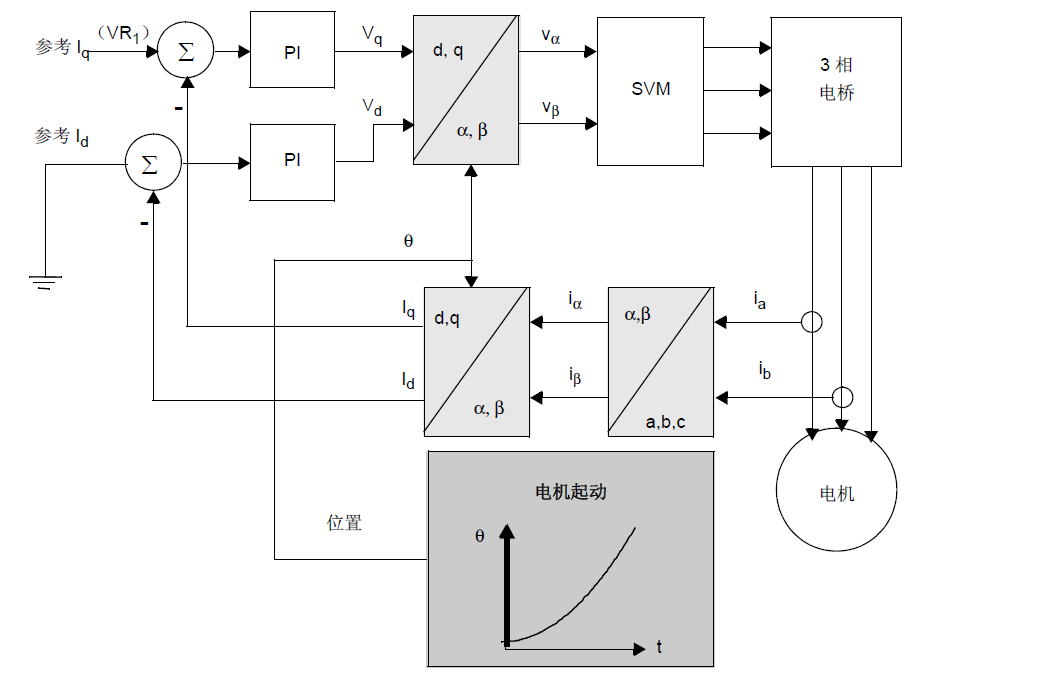
\includegraphics[width=\textwidth]{./picture/IF启动.png}
  \caption{I/F启动控制框图}
  \label{Con1}
\end{figure}

I/F启动的原理即根据期望的速度和加速时间来计算加速度,使得相角度以平方率递增,从而使电机得到一个恒定的加速度。 即使theta 由处于开环状态的电机产生,FOC 电路仍可得到执行并可控制转矩电流分量和磁通电流分量。通过对加速度积分得到电角速度,对电角速度积分得到角度。从而实现电角度频率逐渐增加,从而平稳的将电机拖起,当转子旋转速度达到可观测反电动势时即可切换无感闭环运行。

\subsubsection{滑模控制器}
滑膜观测器的输入量为Vs和is,即两相静止坐标系的α轴和β轴的电压和电流信息,这是由电流采样所获取的电流信息经过clark坐标系变化所得到的。滑膜观测器对电机的转子位置速度信息的估算,是基于电流观测器来实现的。通过电流观测器构建一个虚拟电机模型,
通过实际的电流值和虚拟电机模型的电流值进行比较,比较的输出作为滑动模态控制器的输入,
计算得到一个校正因子Z回馈到虚拟电机模型,从而使得虚拟的电机模型不断接近真实的物理电机模型,通过这种负反馈控制可实现了观测电流收敛于真实电流,从而得到的反电动势信息也收敛于真实的物理系统。
滑膜观测器的电流观测器框图如图\ref{Con_1}所示。
\begin{figure}
  \centering
  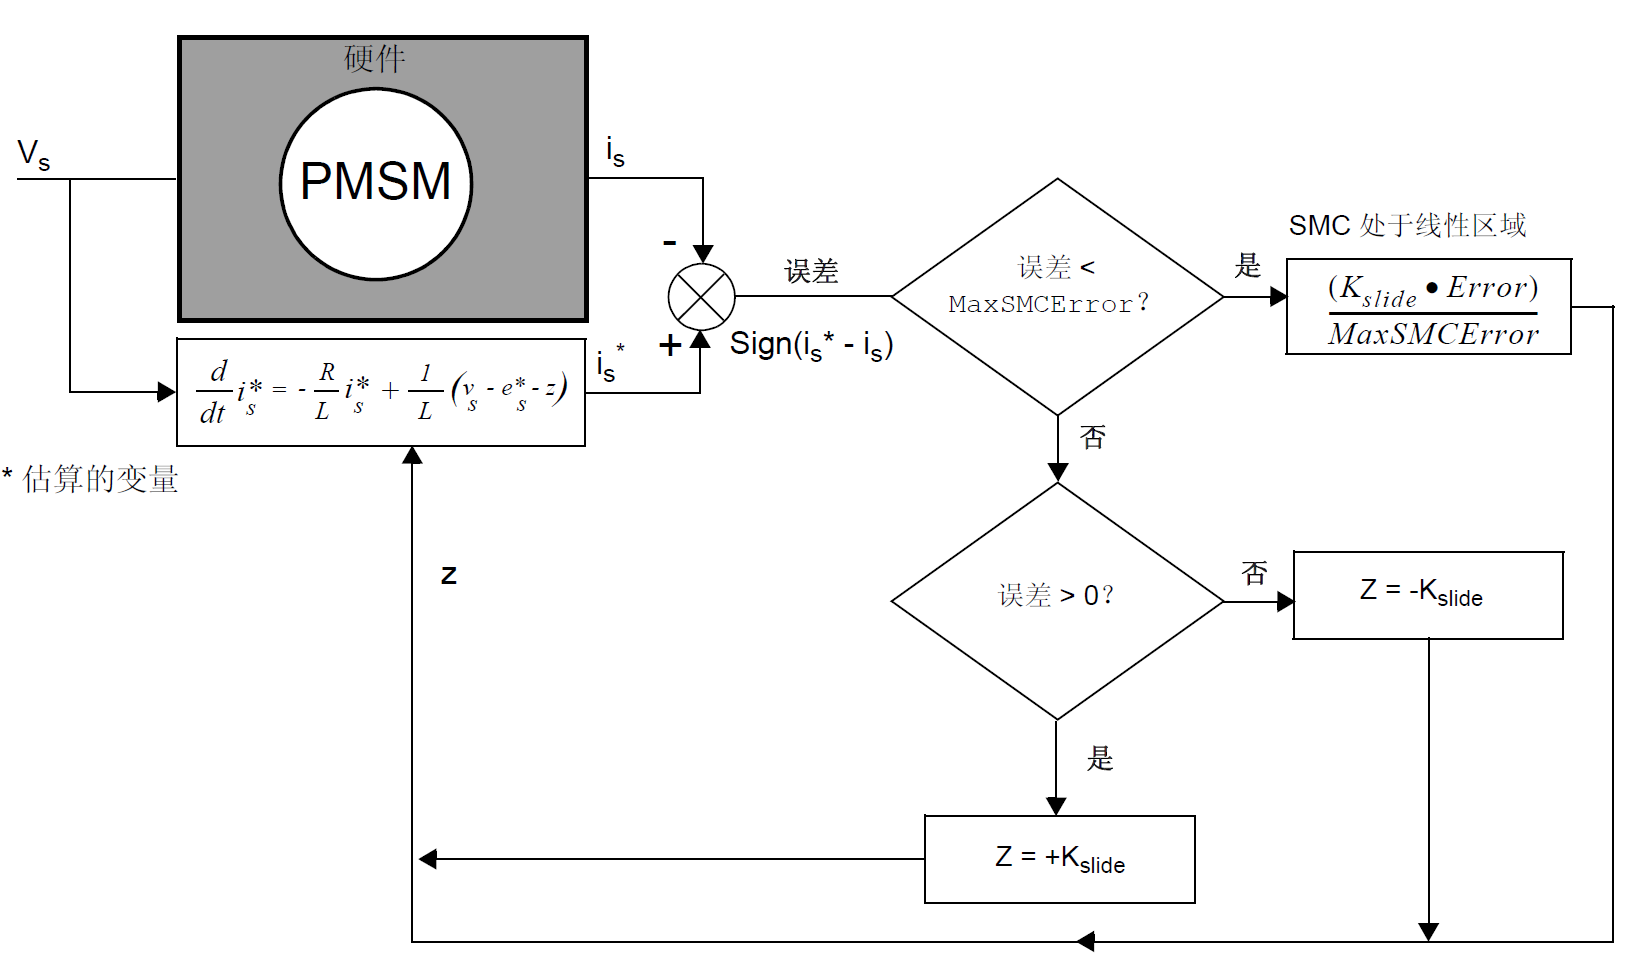
\includegraphics[width=\textwidth]{./picture/滑膜观测器.png}
  \caption{滑膜观测器的电流观测器}
  \label{Con_1}
\end{figure}

电流观测器的模型推导如下:

使用一个直流电机模型来替代电机,该电机模型由绕组电阻、绕组电感和反电动势来表示,如图\ref{Con3}所示。
\begin{figure}
  \centering
  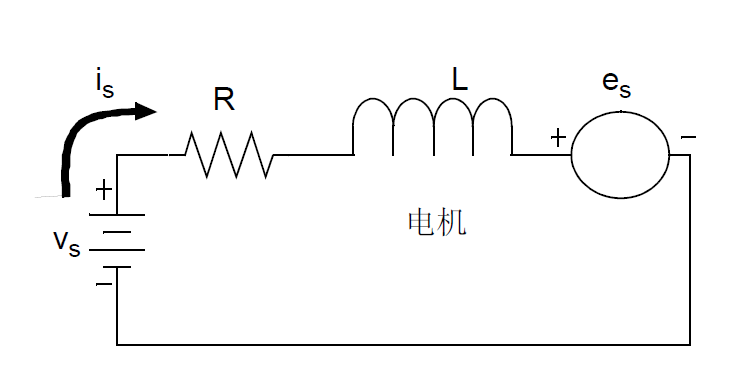
\includegraphics[width=0.5\textwidth]{./picture/电机模型.png}
  \caption{电机模型}
  \label{Con3}
\end{figure}
根据电机模型可得:
\begin{equation}
  v_{s}=R i_{s}+L \frac{d}{d t} i_{s}+e_{s}
\end{equation}
其中$i_{s}$是电机电流矢量,
$v_{s}$是输入电压矢量,
$e_{s}$是反电动势矢量,
$R$为绕组电阻,$L$是绕组电感,
$T_s$是控制周期。
求解$i_s$可得到电机电流:
\begin{equation}
  \frac{d}{d t} i_{s}=\left(-\frac{R}{L}\right) i_{s}+\frac{1}{L}\left(v_{s}-e_{s}\right)
\end{equation}
在数字域中离散化电流方程为:
\begin{equation}
  \frac{i_{S}(n+1)-i_{s}(n)}{T_{S}}=\left(-\frac{R}{L}\right) i_{s}(n)+\frac{1}{L}\left(v_{S}(n)-e_{S}(n)\right)
\end{equation}
求解$i_s$可得:
\begin{equation}
  i_{s}(n+1)=\left(1-T_{s} \bullet \frac{R}{L}\right) i_{s}(n)+\frac{T_{s}}{L}\left(v_{s}(n)-e_{s}(n)\right)
\end{equation}
\begin{equation}
  F=1-T_{s} \bullet \frac{R}{L}
\end{equation}
\begin{equation}
  \mathrm{G}=\frac{\mathrm{T}_{\mathrm{S}}}{\mathrm{L}}
\end{equation}
在电流模型的推导中得到两个参数$G$和$F$,这两个参数为滑膜观测器的增益,需要根据电机的电气信息进行准确修改,才能使得滑膜观测器控制过程中实现收敛。
对于公式中的电感电阻信息可以通过RLC测量仪器进行测量,
这两个信息不仅在滑膜观测器中需要使用,在电机控制电流环设计时也需要使用。

在上图电流观测器框图中,我们可知滑动模态控制器会输出一个校正因子,这个校正因子有两个用途,
一个是用于回馈到电机模型,用以完善电机模型,另一个用途便是估算反电动势\cite{Zhang2022a},
校正因子Z经过一个低通滤波器便可得到反电动势Es,对反电动势进行滤波便可以得到较为干净的反电动势信息,在本项目中我们采用的是反正切的方法来计算转子角度,因此在反电动势经过滤波后便可用反正切来估算转子角度信息。
反电动势估算模型框图如图\ref{Con_2}所示。
\begin{figure}
  \centering
  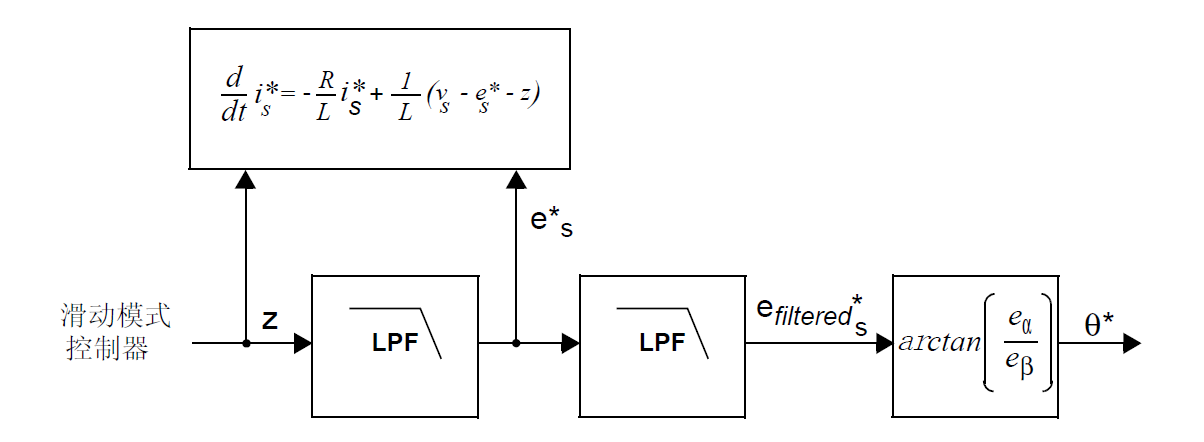
\includegraphics[width=\textwidth]{./picture/反电动势估算模型.png}
  \caption{反电动势估算模型}
  \label{Con_2}
\end{figure}

反电动势估算中所使用的低通滤波器解析如下:
\begin{equation}
  y(n)=y(n-1)+T*2\pi*f_c*(x(n)-y(n))
\end{equation}
前面所讲通过对校正因子Z进行滤波可得到反电动势,在这里我们带入校正因子Z和反电动势说明滤波过程。
\begin{equation}
  e(n)=e(n-1)+(\frac{1}{f_{pwm}})*2\pi*f_c*(z(n)-e(n))
\end{equation}
截止频率的值被设置为等于驱动电流和电机电压的频率,该频率等于每秒的电气旋转圈数。
在估算得到角度信息后便可进行速度信息获取,由于在计算theta 期间应用了滤波函数,所以在使用计算得到的角度给电机绕组通电之前需要对相位进行补偿。
theta 补偿量取决于theta 的变化速率或电机的速度。
theta 补偿由以下两步组成:
\begin{enumerate}
  \item 通过未补偿的theta 来计算电机的速度。
  \item 对计算得到的速度进行过滤,并计算补偿量。
\end{enumerate}

\subsubsection{无感启动过程}
\begin{enumerate}
  \item  START电流模式
        \begin{itemize}
          \item 角度开环(预设角度)、电流闭环
          \item 规划角度和力矩
          \item 判断观测器是否收敛
        \end{itemize}

  \item SWITCH\_OVER电流模式
        \begin{itemize}
          \item 检查能否进入闭环
        \end{itemize}
  \item START\_RUN速度模式
        \begin{itemize}
          \item 设置当前速度为设定速度,目的是平滑过渡。
          \item 判断观测器是否收敛
        \end{itemize}
  \item RUN速度模式
        \begin{itemize}
          \item 角度闭环(估计角度)、速度闭环
        \end{itemize}

\end{enumerate}

% 无传感器控制技术通过估算电机的位置(不使用位置传感器)来实现FOC算法。
% 位置估算器的功能框图如图\ref{Con2}所示。
% \begin{figure}
%   \centering
%   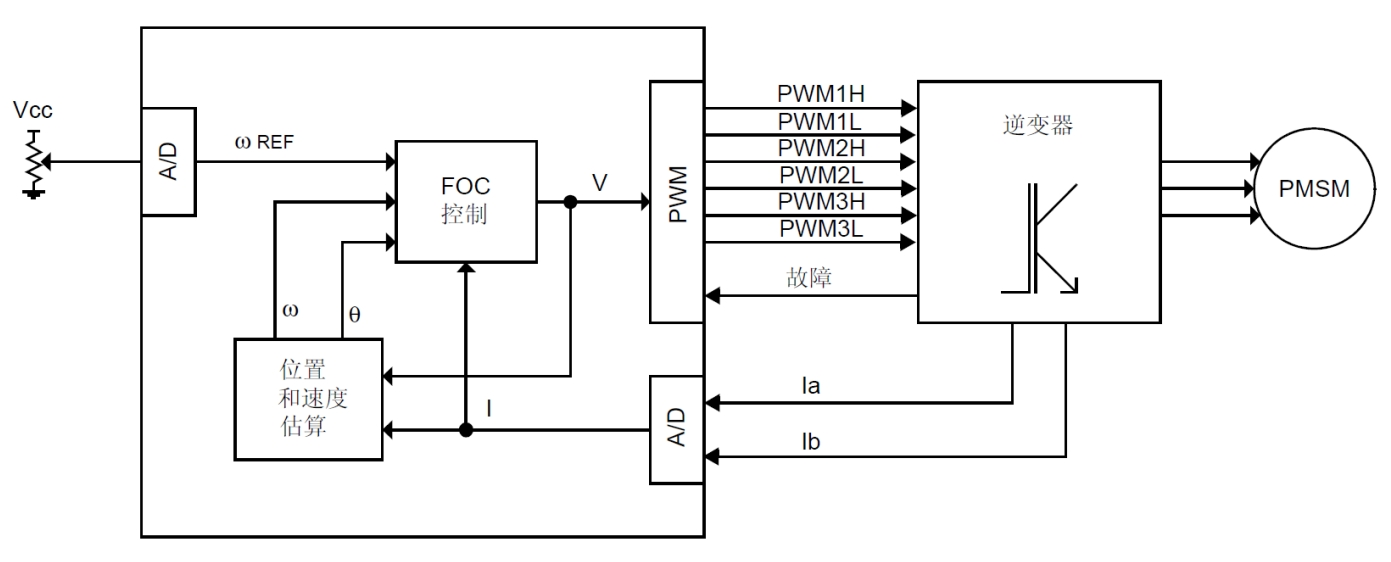
\includegraphics[width=\textwidth]{./picture/无感位置观测.png}
%   \caption{无感位置观测}
%   \label{Con2}
% \end{figure}
% 通过一个直流电机模型来估算PMSM的位置,该电机模型由绕组电阻、绕组电感和反电动势来表示,如图\ref{Con3}所示
% \begin{figure}
%   \centering
%   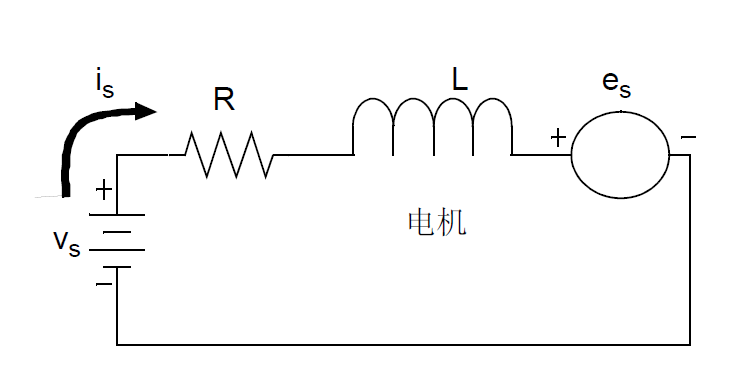
\includegraphics[width=0.5\textwidth]{./picture/电机模型.png}
%   \caption{电机模型}
%   \label{Con3}
% \end{figure}


\subsubsection{电流环控制方案} \label{电流环小节}
电流环采用PID控制,输入量为dq轴参考电流值和实际电流值,在I/F启动阶段,参考电流来自于设定的固定参考电流,用于实现恒力矩拖动电机,当切入到无感闭环运行状态时,电流参考值来自于速度环的输出量。
其控制框图如图\ref{Con5}所示:
\begin{figure}
  \centering
  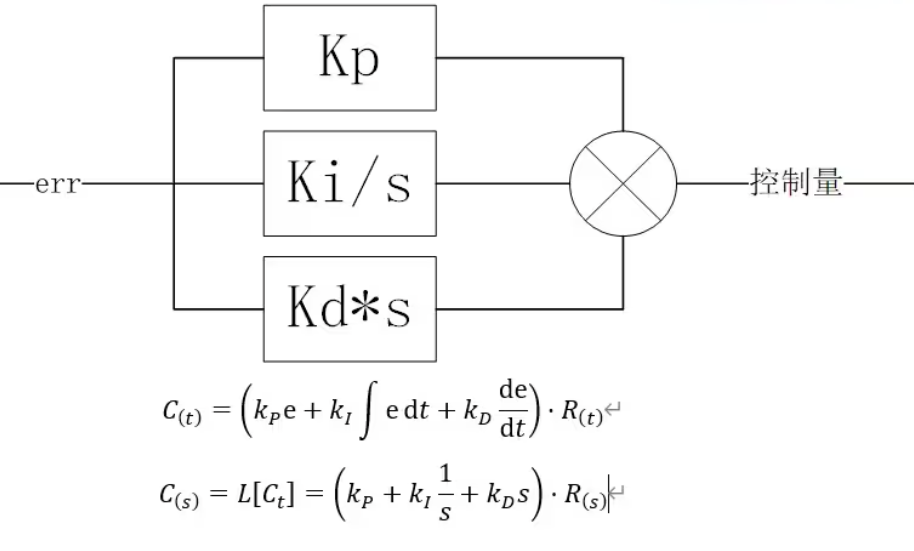
\includegraphics[width=\textwidth]{./picture/电流环.png}
  \caption{电流环控制框图}
  \label{Con5}
\end{figure}


\subsubsection{速度环控制方案}
速度环亦采用PID控制,输入量为用户设定的参考速度于实际估算速度的误差,参考速度可以是手动给定或者通过可调电位器给定,速度环在I/F阶段结束后开启,在I/F阶段是单闭环,即电流闭环,速度开环。

\subsection{有感控制方案}
有感控制方案中的电流环与无感控制中的电流闭环相同,在此不再赘述,详情可见\ref{电流环小节}小节。
本节主要分析有速度传感器条件下的速度闭环、位置闭环及运动控制方案的可行性。
其整体控制框图如下所示。

\subsubsection{速度环控制方案}
本项目有感闭环控制部分使用线性自抗扰控制器(Linear Active Disturbance Rejection Controller, LADRC)。
自抗扰控制器最早由韩京清院士于1989年提出,提出时控制器针对非线性系统描述,其需要整定的参数过多。
高志强教授于2013年在文章\cite{zhiqiang_gao_scaling_2003}中将非线性自抗扰控制器线性化,转化为在工程上易于实现,且控制效果较PID控制器
有明显优势的线性自抗扰控制器,其需要整定的参数仅为3个。
本小节依然从理论出发,逐步推导基于LADRC的永磁同步电机速度环控制方案\cite{Zhong2020},并给出LADRC的参数调整过程,
其参数调整过程对工程实践具有指导意义。

基于式(\ref{DModel_3}), 转速环节的微分方程表示如式 (\ref{DModel_4}):
\begin{equation}
  \label{DModel_4}
  \frac{d\omega}{dt}=\frac{1}{J}(1.5p\psi_{f}i_{q}-T_L-B\omega)
\end{equation}
为了将其转化为一个完整的级联系统,可以将其转换为 (\ref{DModel_5}):
\begin{equation}
  \label{DModel_5}
  \frac{d\omega}{dt}=b_0i_q^{\ast}+f_w
\end{equation}
其中 $f_w$ 是包含外扰和内扰的总体扰动:
\begin{equation}
  \label{DModel_6}
  f_w = \frac{1}{J}(1.5p\psi_{f}i_{q}-T_L-B\omega)-b_0i_q^{\ast}
\end{equation}
令$x_1=w_r$,$x_2=f_w$,$u=i_q^{\ast}$,那么(\ref{DModel_6}) 可以转化为(\ref{LADRC_1}):
\begin{equation}
  \label{LADRC_1}
  \left\{\begin{array}{l}
    \dot{x}=Ax+Bu+Eh \\
    y=Cx
  \end{array}\right.
\end{equation}
其中 $A = \begin{bmatrix}
    0 & 1 \\
    1 & 1
  \end{bmatrix}$,
$B = \begin{bmatrix}
    b_0 \\
    1
  \end{bmatrix}$,
$E = \begin{bmatrix}
    0 \\
    1
  \end{bmatrix}$,$h=\dot{f_w}$,$C=[1\quad 0]$.LESO根据(\ref{LADRC_1})被设计成(\ref{LADRC_2}) :
\begin{equation}
  \label{LADRC_2}
  \left\{\begin{array}{l}
    \dot{z}=Ax+Bu+L(y-(\hat{y})) \\
    \hat{y}=Cz
  \end{array}\right.
\end{equation}
其中 $L=\begin{bmatrix}
    \beta_1 \\
    \beta_2
  \end{bmatrix}$。由此,基于上述推导可画出永磁同步电机的LADRC控制框图:

\begin{figure}[ht]
  \centering
  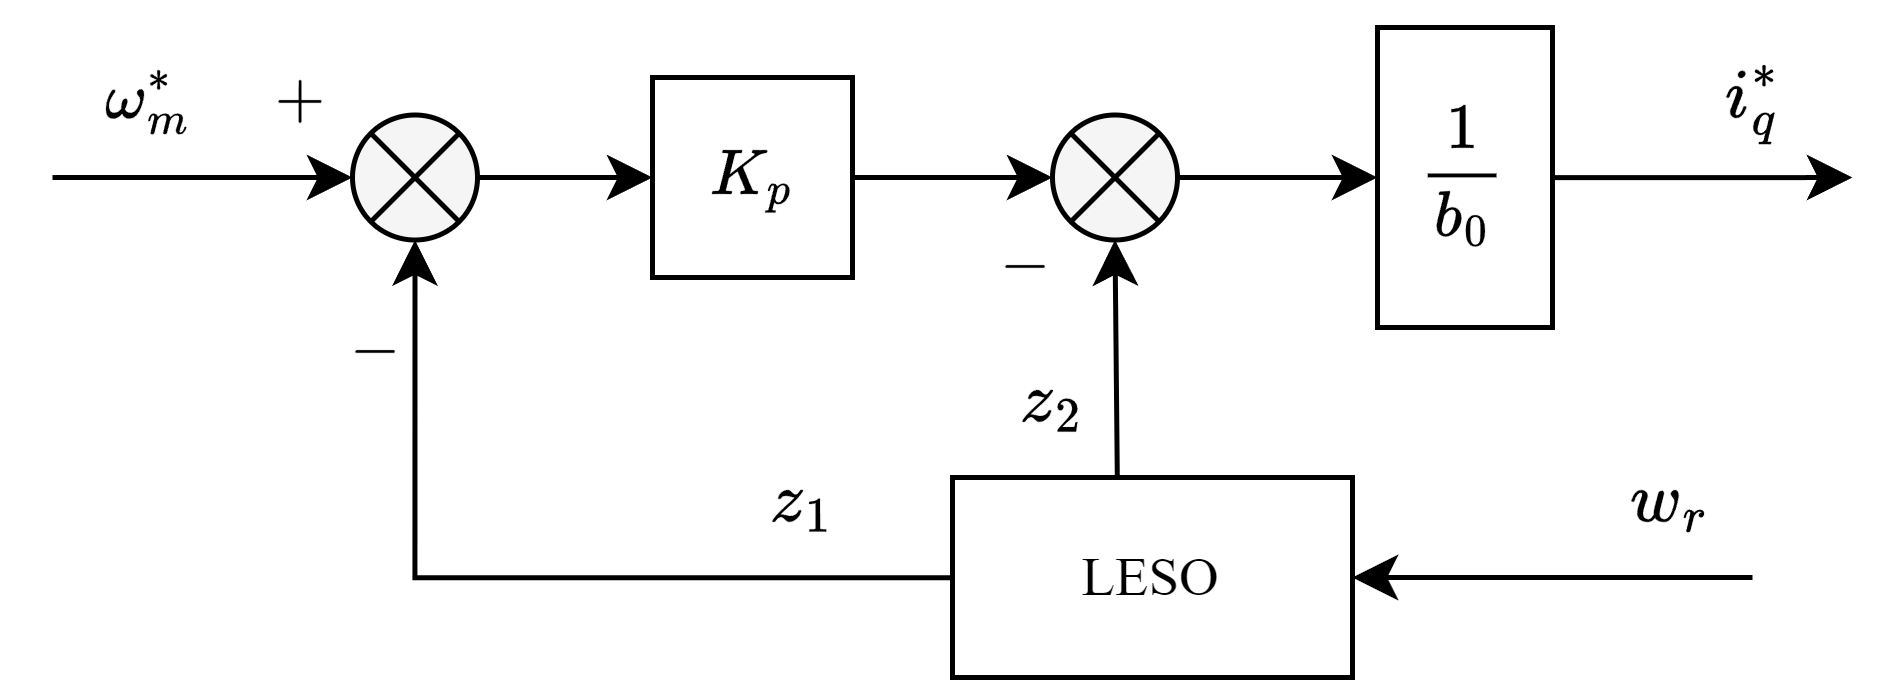
\includegraphics[width=0.5\textwidth]{./picture/LADRC控制框图.png}
  \caption{永磁同步电机的LADRC控制框图}
  \label{LADRC}
\end{figure}


采用\cite{zhiqiang_gao_scaling_2003}中的带宽法来确定观测器的增益,可得$\beta_1=2\omega_o$,$\beta_2=\omega_o^2$。
其中$\omega_o$为观测器带宽。
LADRC通过观测器补偿速度误差。
观测器对误差的跟随速度取决于线性扩展观测器的带宽。
带宽越大,对误差的观测越即时,但同时,大带宽会引入噪声,严重时会使系统震荡。
因此,如何通过选定带宽参数$\omega_o$使观测器保持较高带宽,同时不引入噪声是一个值得探讨的问题。

由上述推导可知,LADRC控制器有3个参数需要整定,分别为$\omega_o$,$K_p$和$b_0$。
在本项目中,三参数整定过程如下:
\begin{enumerate}
  \item 标定$b_0$,在电流闭环模式下,给定$q$轴参考电流,观测电机的加速度曲线,根据公式计算得到$b_0$。
  \item 初步标定$w_0$,使用无感控制中的速度环PI控制器,将滑模观测器估计值替换为速度传感器值。
        在此PI观测器中,不对速度响应质量有要求,电机速度有跟随趋势即可。此时调节$w_0$,使观测速度能够跟随电机速度。
  \item 标定$K_p$,此时,在控制器中取消LESO的$z_2$补偿部分,单独调节$K_p$,使电机速度能够快速跟随参考速度值。
  \item 再次标定$w_0$,此时,恢复控制器中LESO的$z_2$补偿部分。微调$w_0$,使电机对参考速度的瞬态响应和稳定响应达到最佳。
\end{enumerate}


\subsubsection{位置环控制方案}
此项目中,位置环采用具有速度限制的单P控制。可调整参数为速度限制值和单P。

\subsubsection{运动控制方案}
为满足机器人关节在实际应用场景中的运功控制需求,即在目标时刻达到目标位置,
本项目采用三次多项式规划进行电机运动轨迹生成。
设电机位置随时间变化的函数为$\theta(t)$。
为了获得一条确定的光滑轨迹曲线,需要对$\theta(t)$施加4个约束条件,
即初始时刻电机速度为零$\dot{\theta}(0) = 0$,结束时刻电机速度为零$\dot{\theta}(t_{end}) = 0$,
初始位置为当前位置$\theta(0) = \theta_0$,结束位置为目标位置$\theta(0) = \theta_f$。
多项式次数至少为3才能满足4个约束条件,该三次多项式具有如下形式:
\begin{equation}
  \label{motion-1}
  \theta(t)=a_0+a_1t+a_2t^2+a_3t^3
\end{equation}
其中$a_0$,$a_1$,$a_2$,$a_3$分别为三次多项式的系数。
则对于指定轨迹的速度曲线显然为:
\begin{equation}
  \label{motion-2}
  \dot{\theta}(t)=a_1+2a_2t+3a_3t^2
\end{equation}
将上述4个条件代入式(\ref{motion-1})和式(\ref{motion-2})可得到含有4个未知量的4个方程:
\begin{align}
  \left\{
  \begin{aligned}
     & \theta_0=a_0                          \\
     & \theta_f=a_0+a_1t_f+a_2t_f^2+a_3t_f^3 \\
     & 0 = a_1                               \\
     & 0 = a_1+2a_2t_f+3a_3t_f^2
  \end{aligned}
  \right.
\end{align}
解出方程中的$a$,可以得到:
\begin{align}
  \label{motion-3}
  \left\{
  \begin{aligned}
     & a_0 = \theta_0                            \\
     & a_1=0                                     \\
     & a_2 = \frac{3}{t_f^2}(\theta_f-\theta_0)  \\
     & a_3 = -\frac{2}{t_f^3}(\theta_f-\theta_0)
  \end{aligned}
  \right.
\end{align}
应用式(\ref{motion-3})可以求出从任何起始角度到终止角度的三次多项式,以此完成电机的运动控制。

\newpage
\section{电路原理分析与电路图}
本项目的硬件连接框图如图\ref{board1}所示,GD32通过IIC控制OLED模块,通过SPI与电机驱动模块中的DRV8301芯片通信,
并通过PWM控制电机驱动板,GD32通过IIC读取AS5600磁编码器,编码器与电机通过机械结构进行连接。
本项目中,我们制作了两块电路板,分别为电机驱动电路板和AS5600编码器电路板,接下来对这两块电路板进行详细说明。
\begin{figure}[ht]
  \centering
  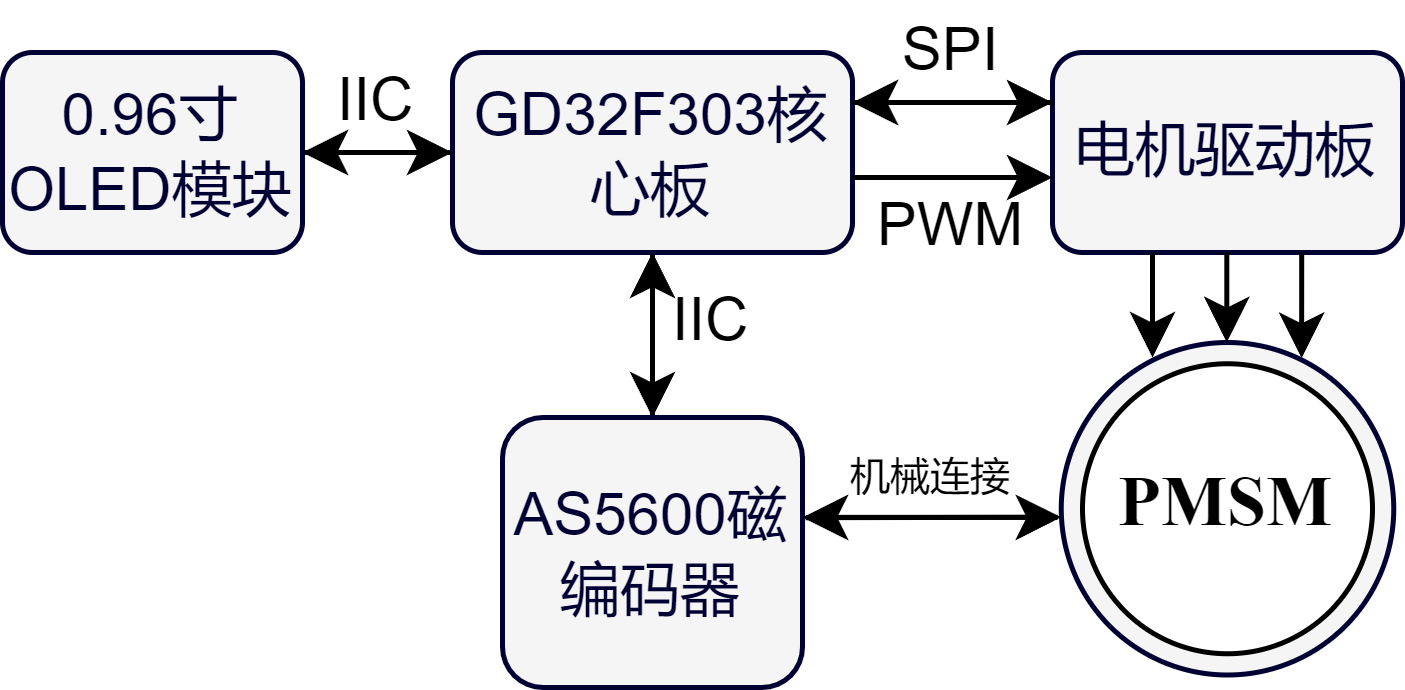
\includegraphics[width=0.5\textwidth]{./picture/硬件电路总体框图.drawio.png}
  \caption{硬件电路总体架构图}
  \label{board1}
\end{figure}


\subsection{电机驱动板}
电机驱动板总原理图如图\ref{board2}所示,其PCB图如图\ref{board3}所示,
其PCB实物图如图\ref{boardx}所示。
电机驱动板由电机驱动芯片drv8301,6个MOS管组成的三相逆变电路和其他外围电路组成。
\begin{figure}[!h]
  \centering
  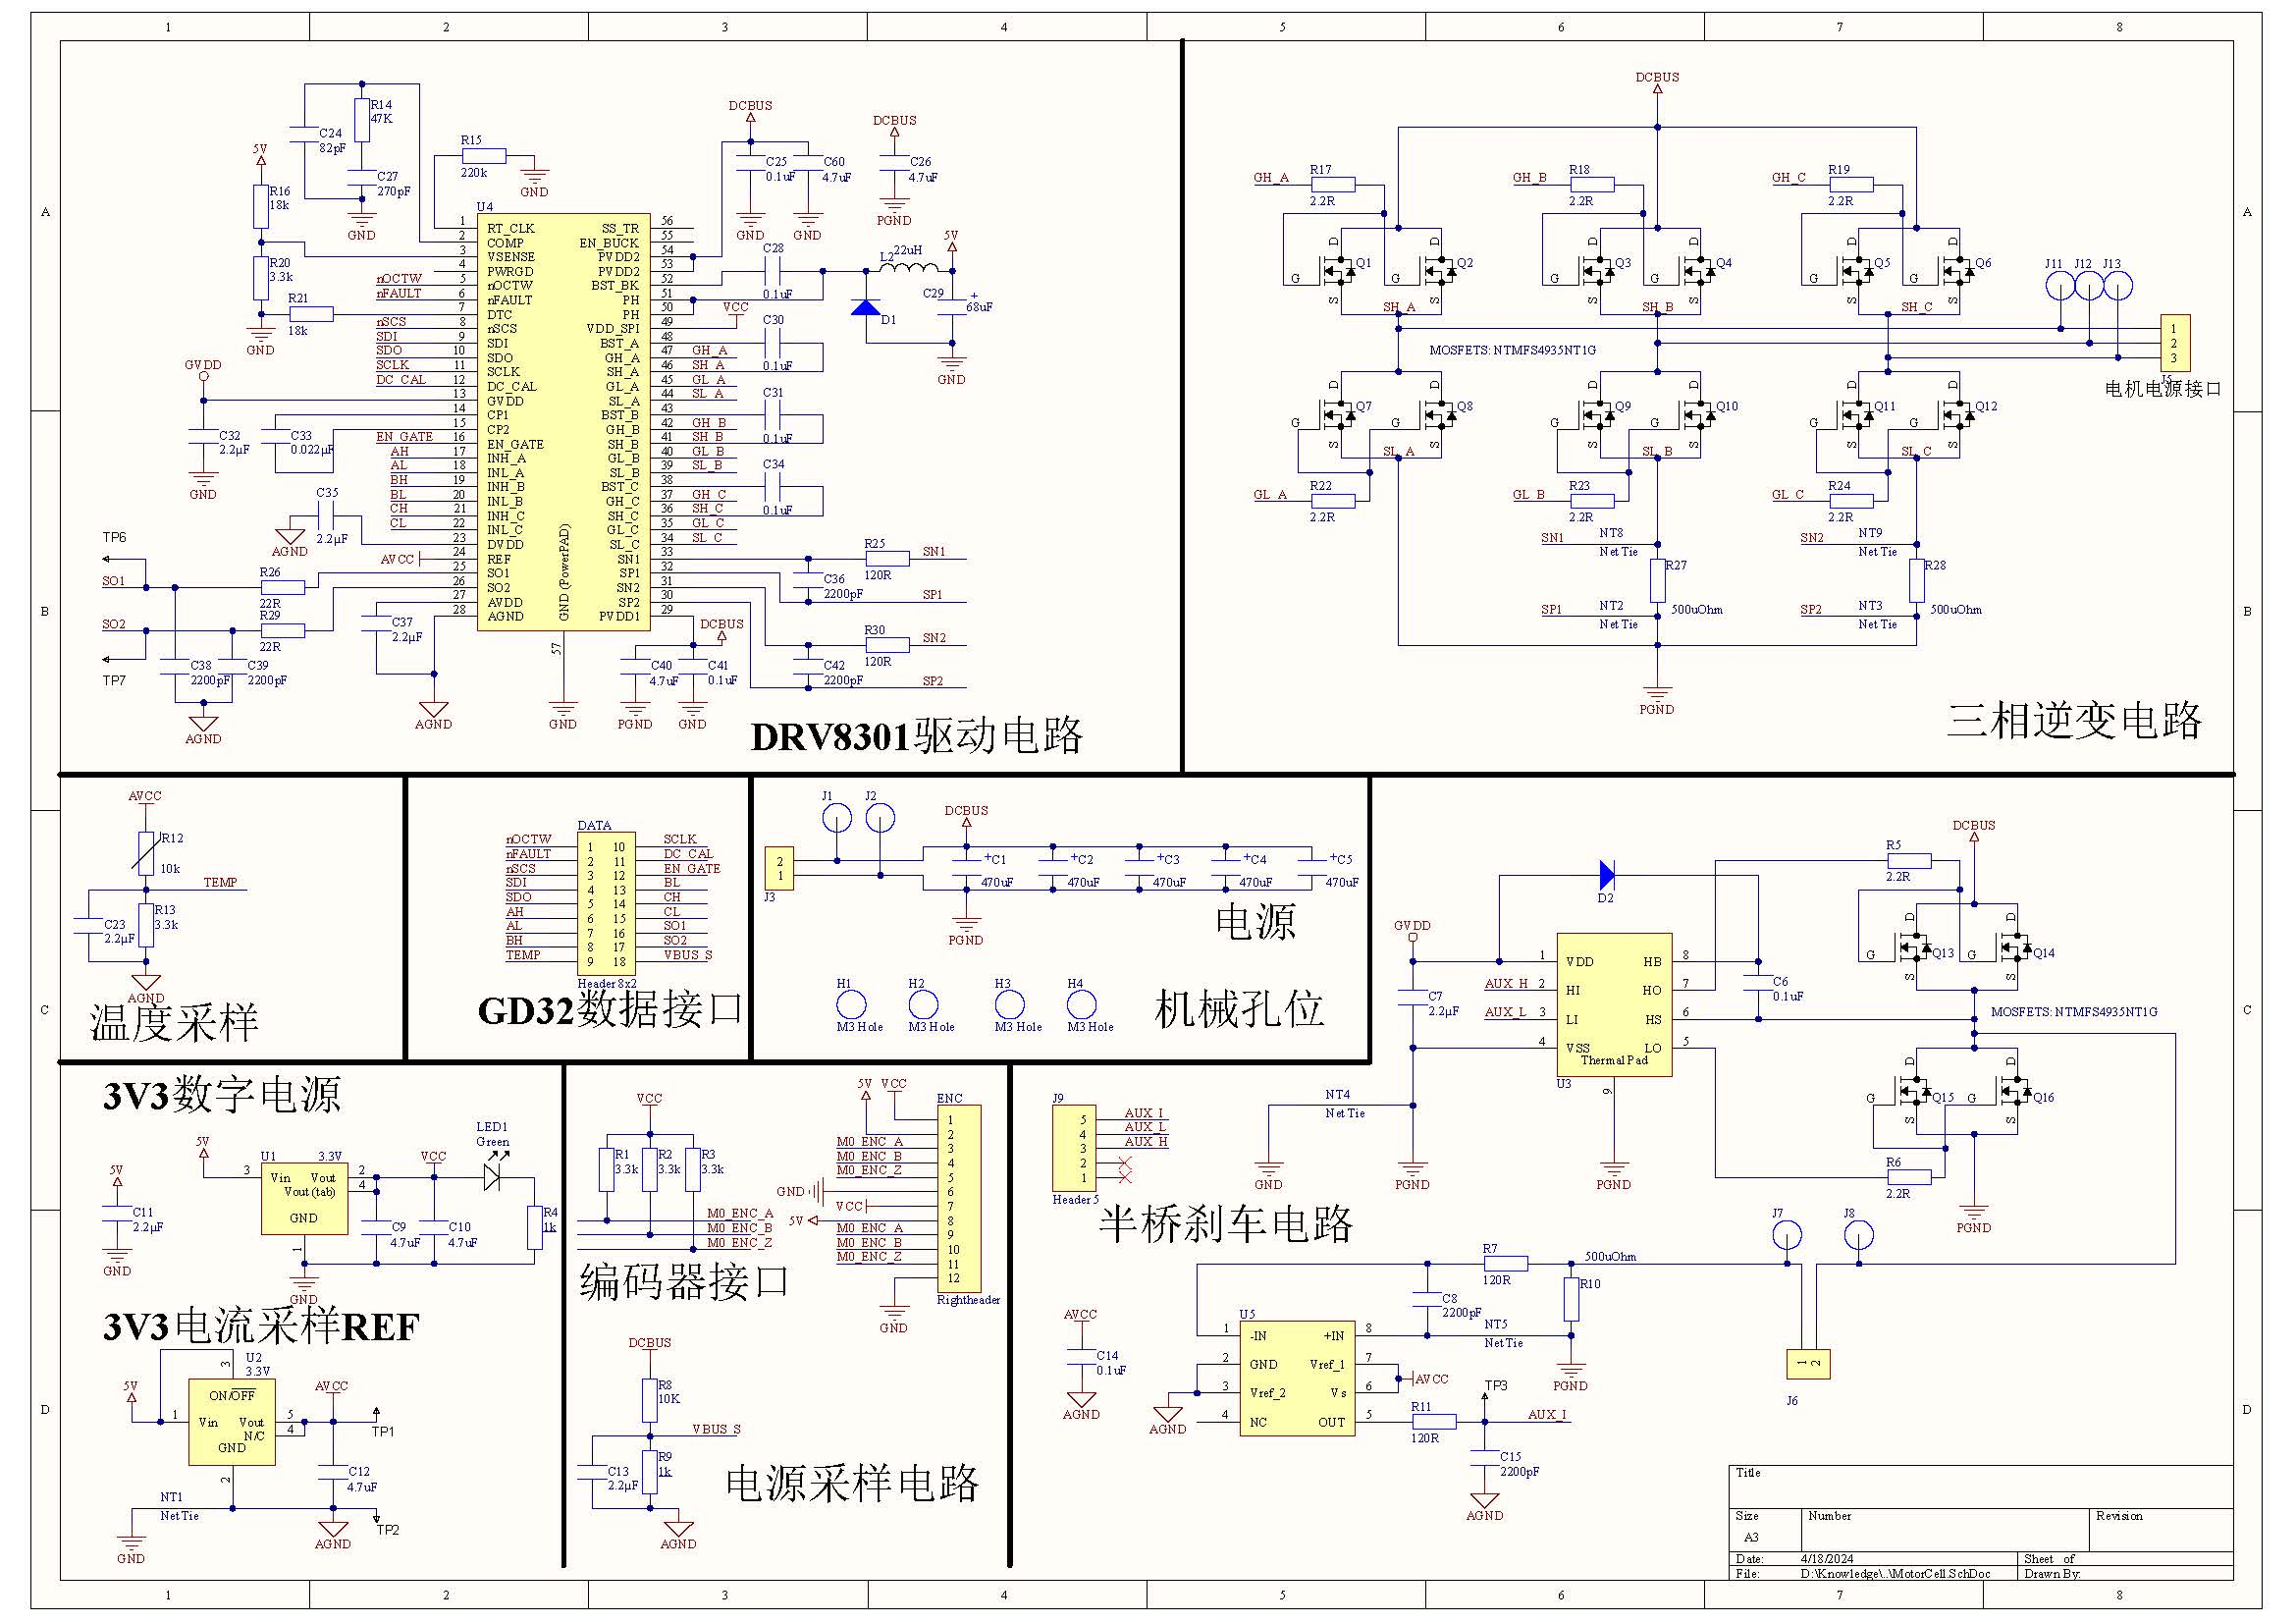
\includegraphics[width=\textwidth]{./picture/GDriver_Seperate_页面_1.jpg}
  \caption{电机驱动原理总图}
  \label{board2}
\end{figure}
\begin{figure}[!h]
  \centering
  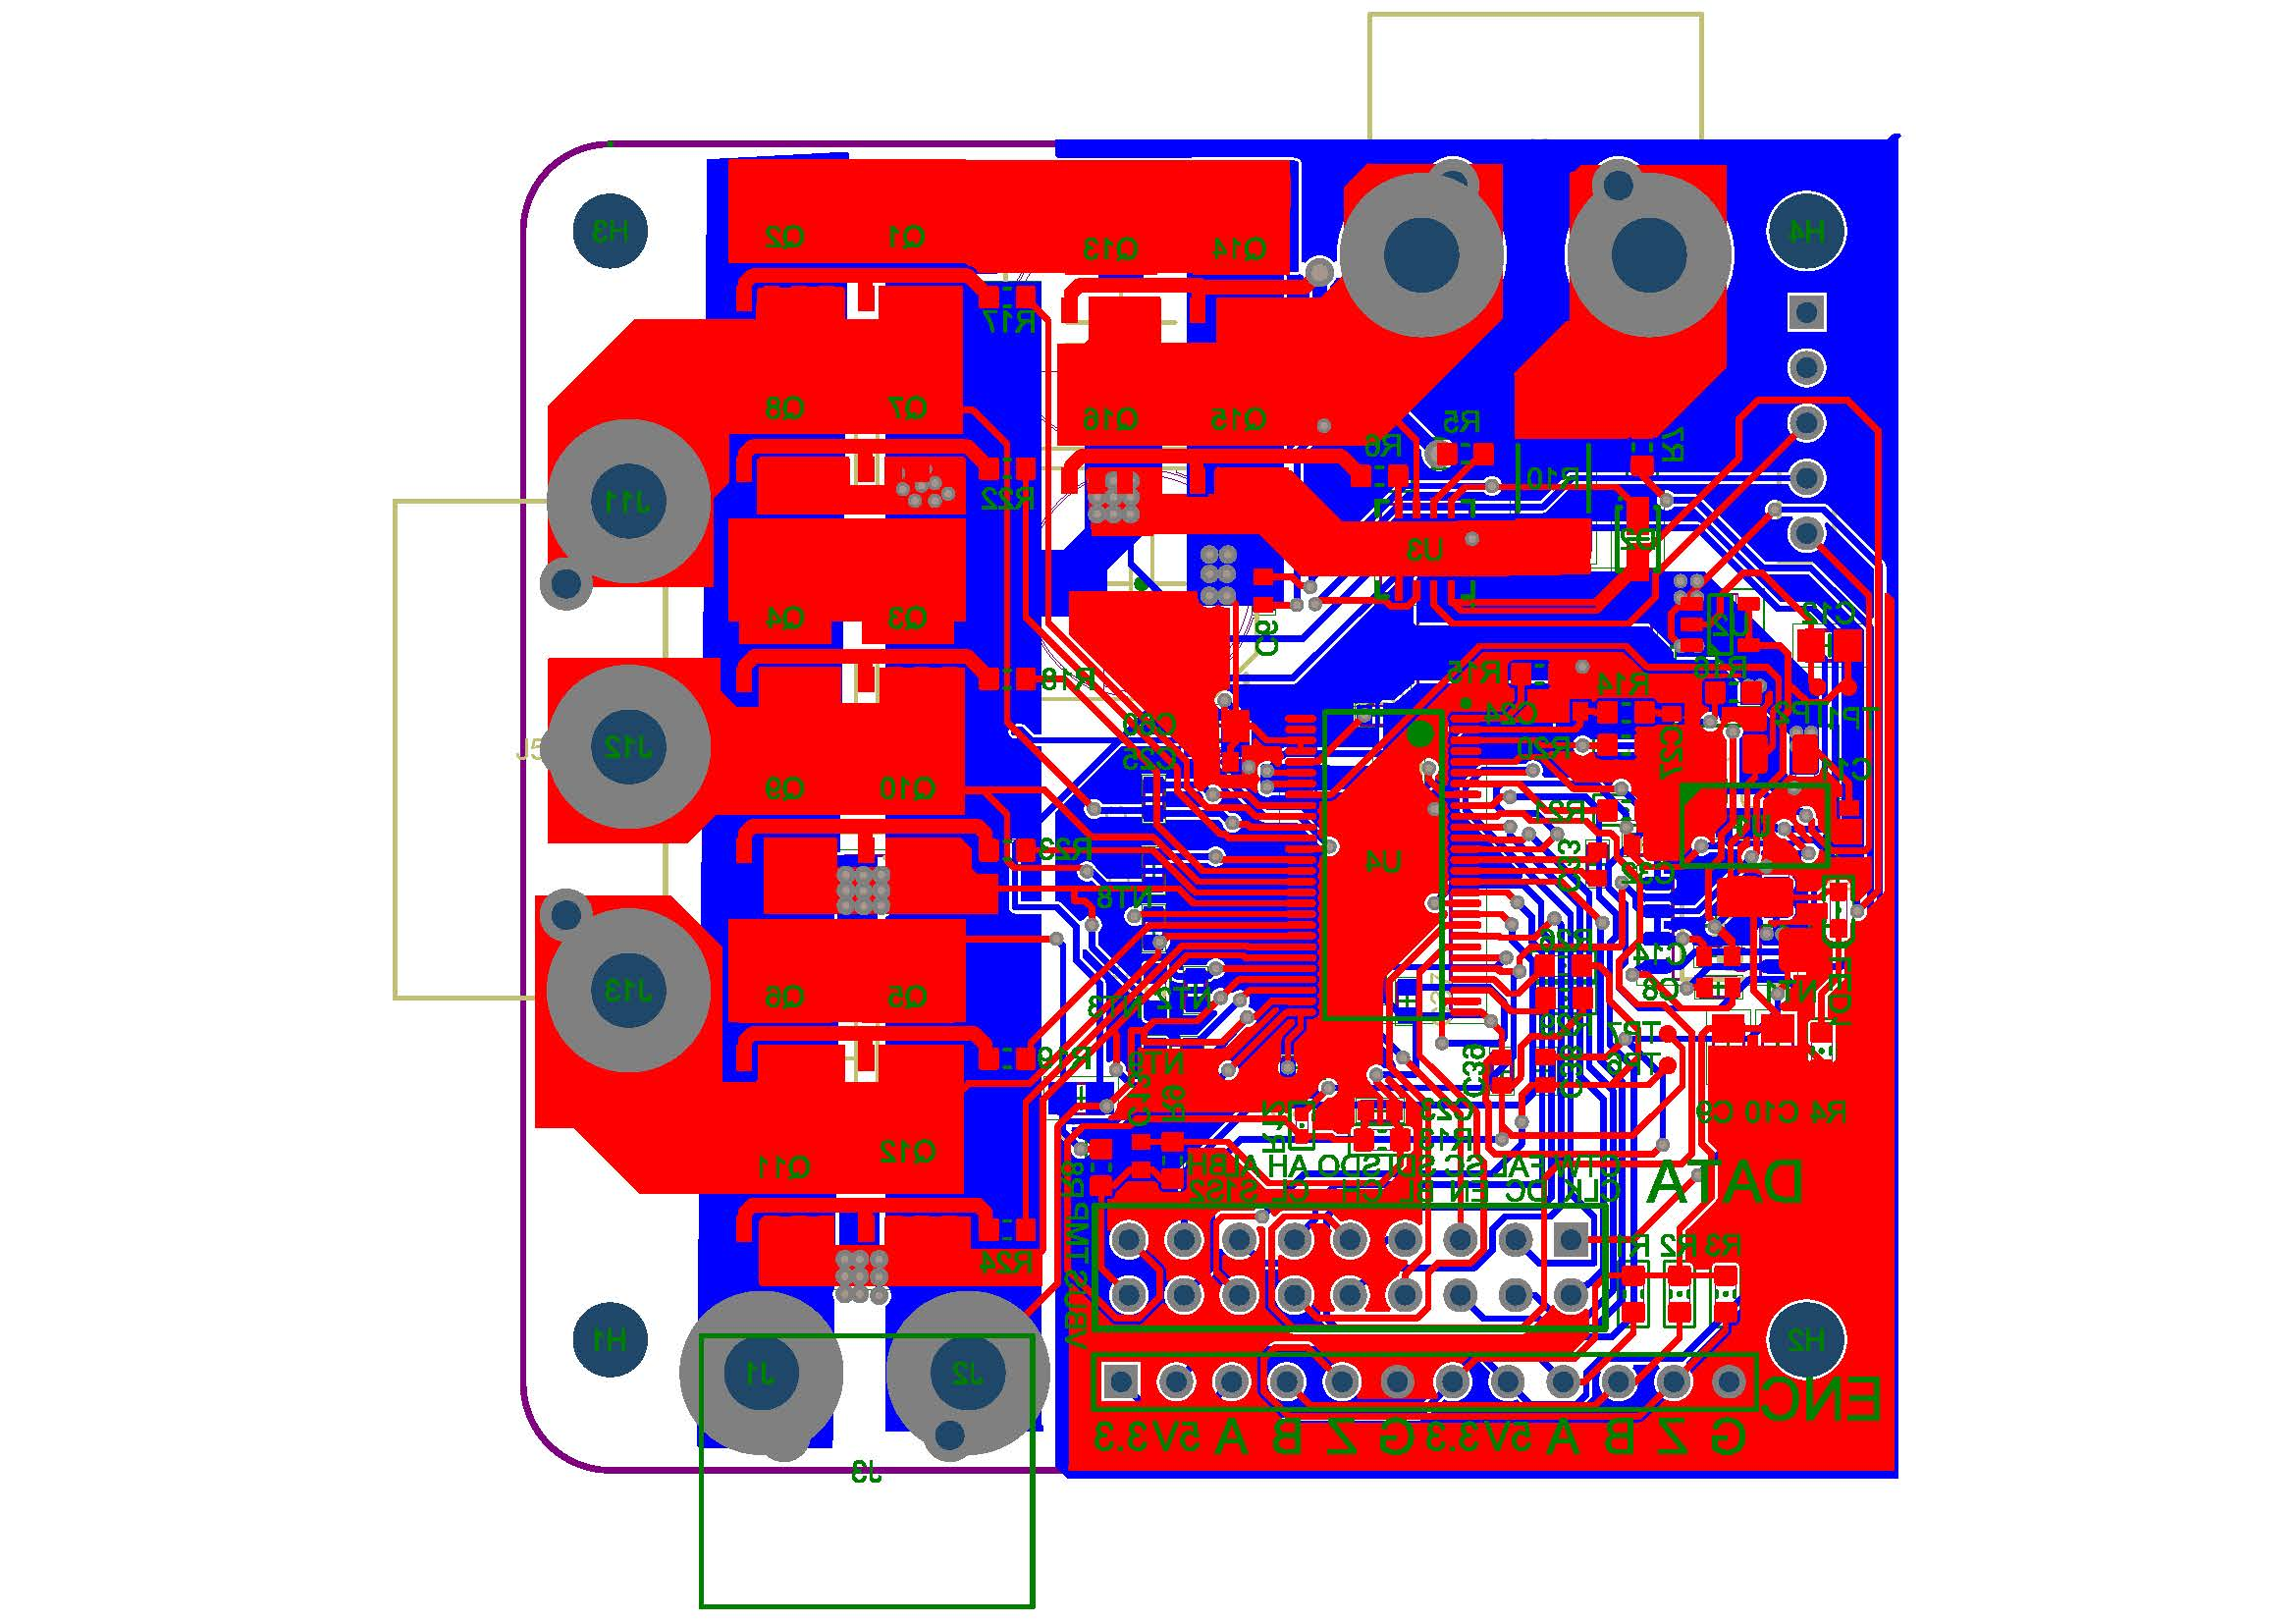
\includegraphics[width=\textwidth]{./picture/GDriver_Seperate_页面_2.jpg}
  \caption{电机驱动电路PCB图}
  \label{board3}
\end{figure}
\begin{figure}[!h]
  \centering
  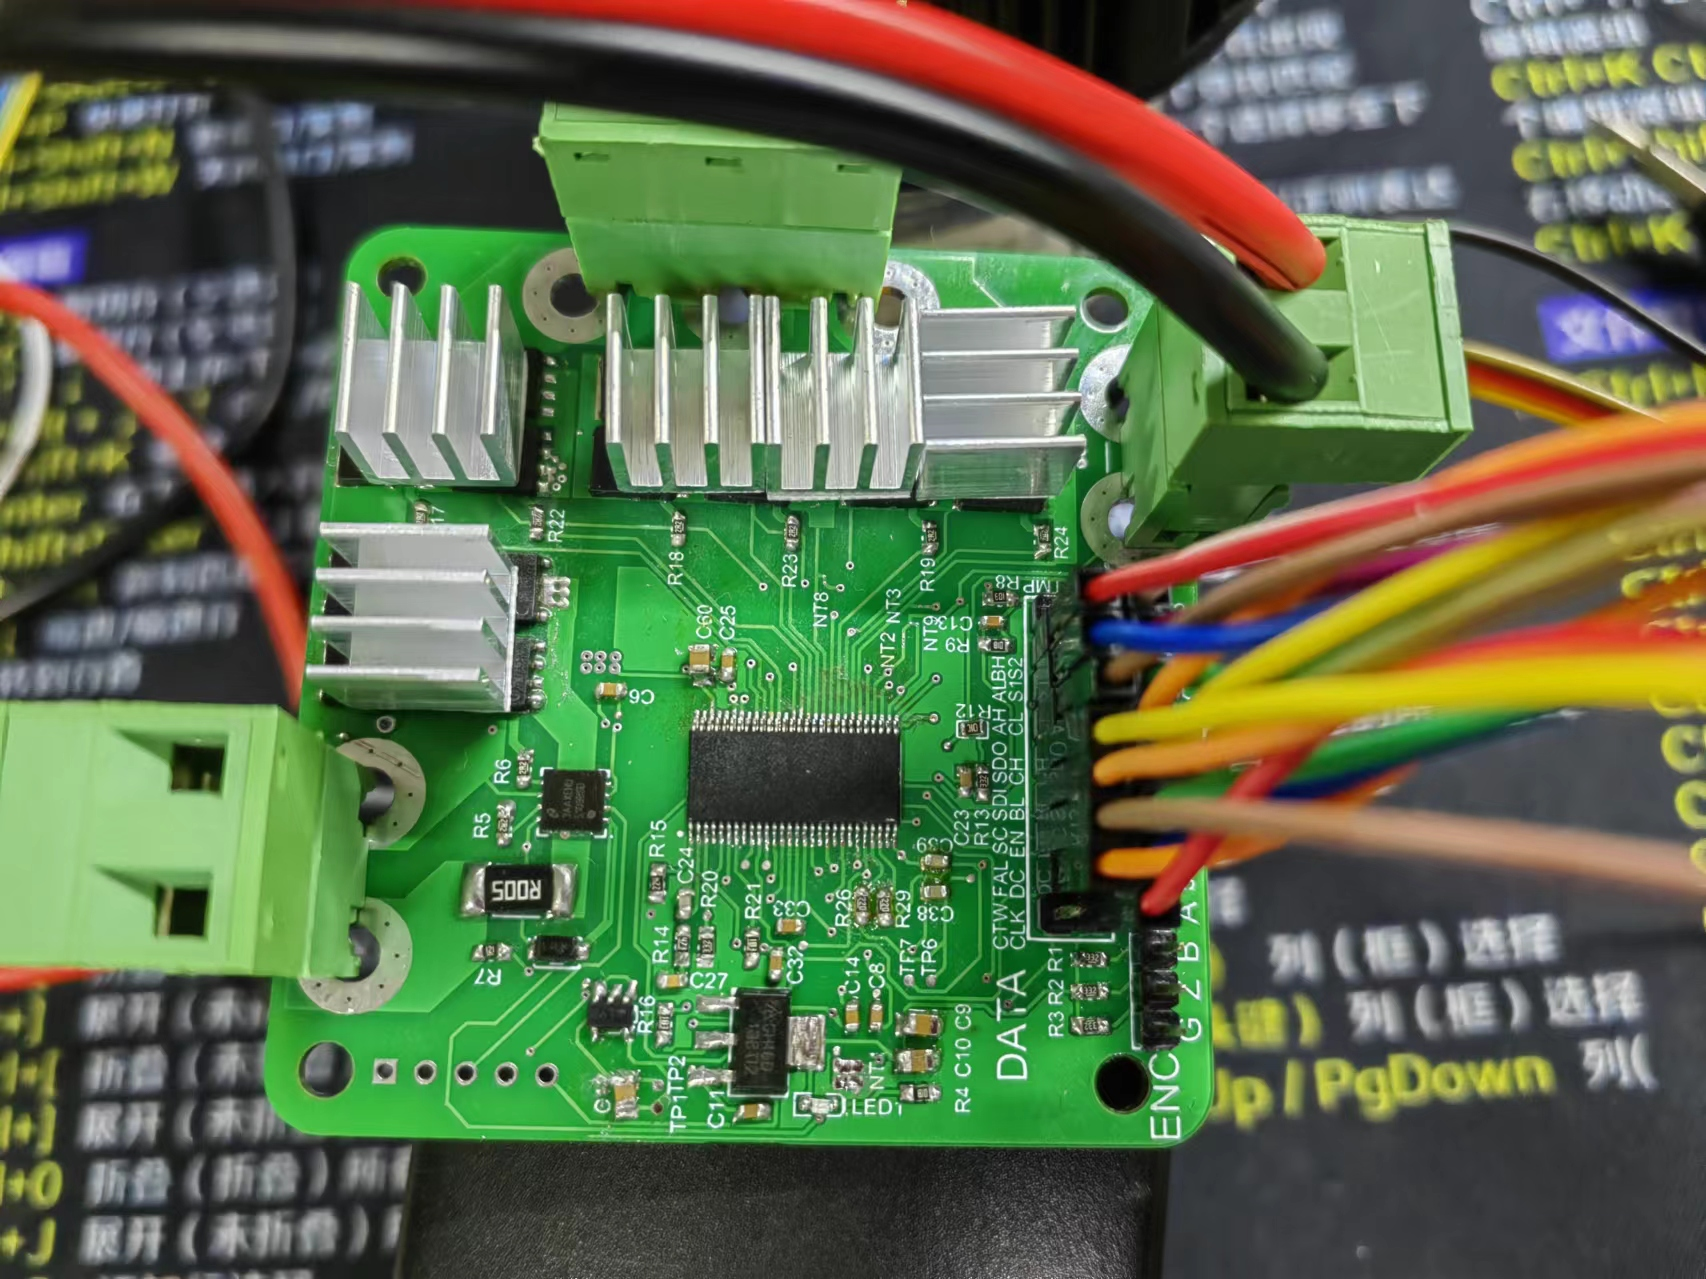
\includegraphics[width=\textwidth]{./picture/电机驱动板.jpg}
  \caption{电机驱动电路实物图}
  \label{boardx}
\end{figure}


\subsubsection{电机驱动芯片电路}
DRV8301是一款集电流采样,全桥驱动,过流保护等功能的电机驱动芯片。
在本设计中,使用DRV8301的内置BUCK降压型电路输出5V电压,
再分别通过AZ1117和LP5907两个LDO降压芯片将5V降压至3.3V,这两个3.3V电源分别为电机驱动板的数字电源和模拟电源。
数字电源对数字型器件供电,如编码器,GD32核心板等。
模拟电源则对模拟器件供电,如作为DRV8301电流采样电路的基准电压及电流采样芯片供电。

\subsubsection{半桥刹车电路}
半桥刹车电路由一个半桥驱动芯片LM5109,两个MOS管组成的开关电路和一个电流采样芯片AD8418组成。
通过外接刹车电阻来实现能量耗散,在保证电路安全的前提下快速刹车的目的。
在实际使用电机驱动板时,需要自行选择刹车电阻的阻值和功率。
刹车电阻通常不需要太大,可选用10欧姆,20欧姆,100欧姆。
刹车电阻阻值越小,刹车速度越快。
刹车电阻的功率应根据电机的实际运行需求来选取,例如已知刹车电流$I$为2安培,此时选用20欧姆的刹车电阻$R$,
那么此时电阻应耗散的功率$P$为:
\begin{equation}
  \label{board4}
  P = I^2R=80W
\end{equation}
那么可以选择功率大于等于80瓦的刹车电阻。
刹车电阻下方通过一个0.5毫欧的采样电阻对电流进行采样,
经过AD8418转换后,经过R11和C15组成的RC低通滤波器输出给GD32。
在电机运转过程中,由GD32采样电流来决定是否开启刹车电阻(耗散电阻)来保护电路。


\subsubsection{其他电路与PCB布局布线说明}
为使驱动器稳定运行,除基本功能电路外,还添加了滤波电路,温度检测电路等,说明如下:
\begin{itemize}
  \item 电源滤波电路:为抑制电源纹波,使用5个470uF的贴片电解电容进行滤波,该滤波电容能有效缓解电压冲击,使电路板稳定运行。
  \item 电源电压检测电路:使用两电阻分压,使GD32能读取电机驱动板供电电压,从而完成低压预警等功能。
  \item 温度采样电路:通过两电阻分压,使GD32能读取热敏电阻近地端电压,将该热敏电阻放置在某一MOS管附近,以此实现温度检测功能。
\end{itemize}

PCB布局布线过程中,将电机的三相接口和电源接口均做敷铜处理,以尽可能大地增大散热面积,使电路能承载大电流工况。
同时针对数字地和电源地进行隔离处理,增强电路稳定性。


\subsection{磁编码器电路板}
磁编码器采用AS5600芯片制作,提供了两种模式的输出接口,I2C和模拟量输出两种。
尺寸契合电机,可以直接安装于电机上。
编码器电路板实物图如图\ref{cibian}所示。
\begin{figure}[htbp]
  \centering
  \begin{minipage}{0.3\linewidth}
    \centering
    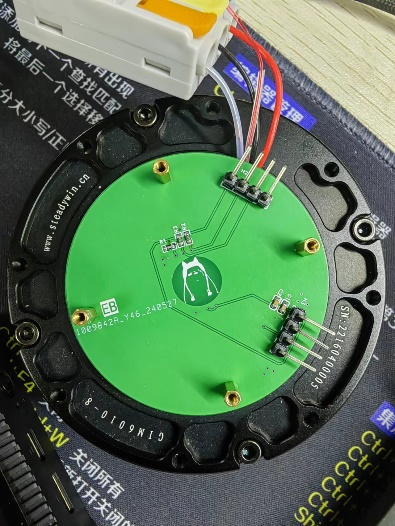
\includegraphics[width=\linewidth]{picture/编码器1.png}
    \caption{编码器安装于电机实物图}
  \end{minipage}
  \begin{minipage}{0.3\linewidth}
    \centering
    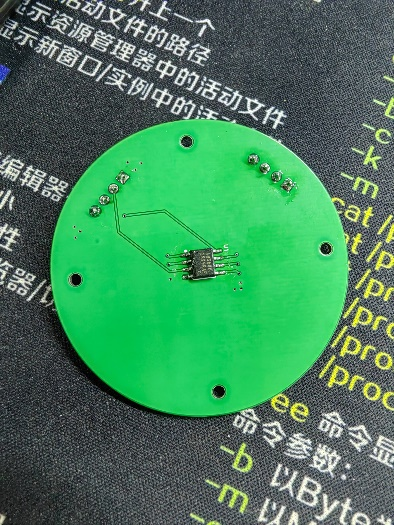
\includegraphics[width=\linewidth]{picture/编码器2.png}
    \caption{编码器背面图}
  \end{minipage} 	%\qquad	%让图片换行,
  \caption{编码器电路板实物图}
  \label{cibian}%文中引用该图片代号
\end{figure}

\clearpage

\newpage
\section{程序设计}
本驱动器所有功能均在GD32F303ZET6单片机上实现,其整体程序框架如图\ref{software1}所示。
驱动层使用了模数转换模块ADC,单片机内部定时器TIM,基于定时器的PWM输出,由GPIO模拟出的IIC和SPI通信接口以及单片机UART接口(串口)。
应用层包含基于ADC的电压与温度采样模块,基于PWM的全桥驱动电路控制模块,基于IIC的OLED显示和编码器角度读取模块,基于SPI的DRV8301驱动模块和基于串口的指令解析与状态机跳转模块。
为满足算法运行时严格的时序要求,算法层中全部算法在定时器中断中运行。
\begin{figure}[!h]
  \centering
  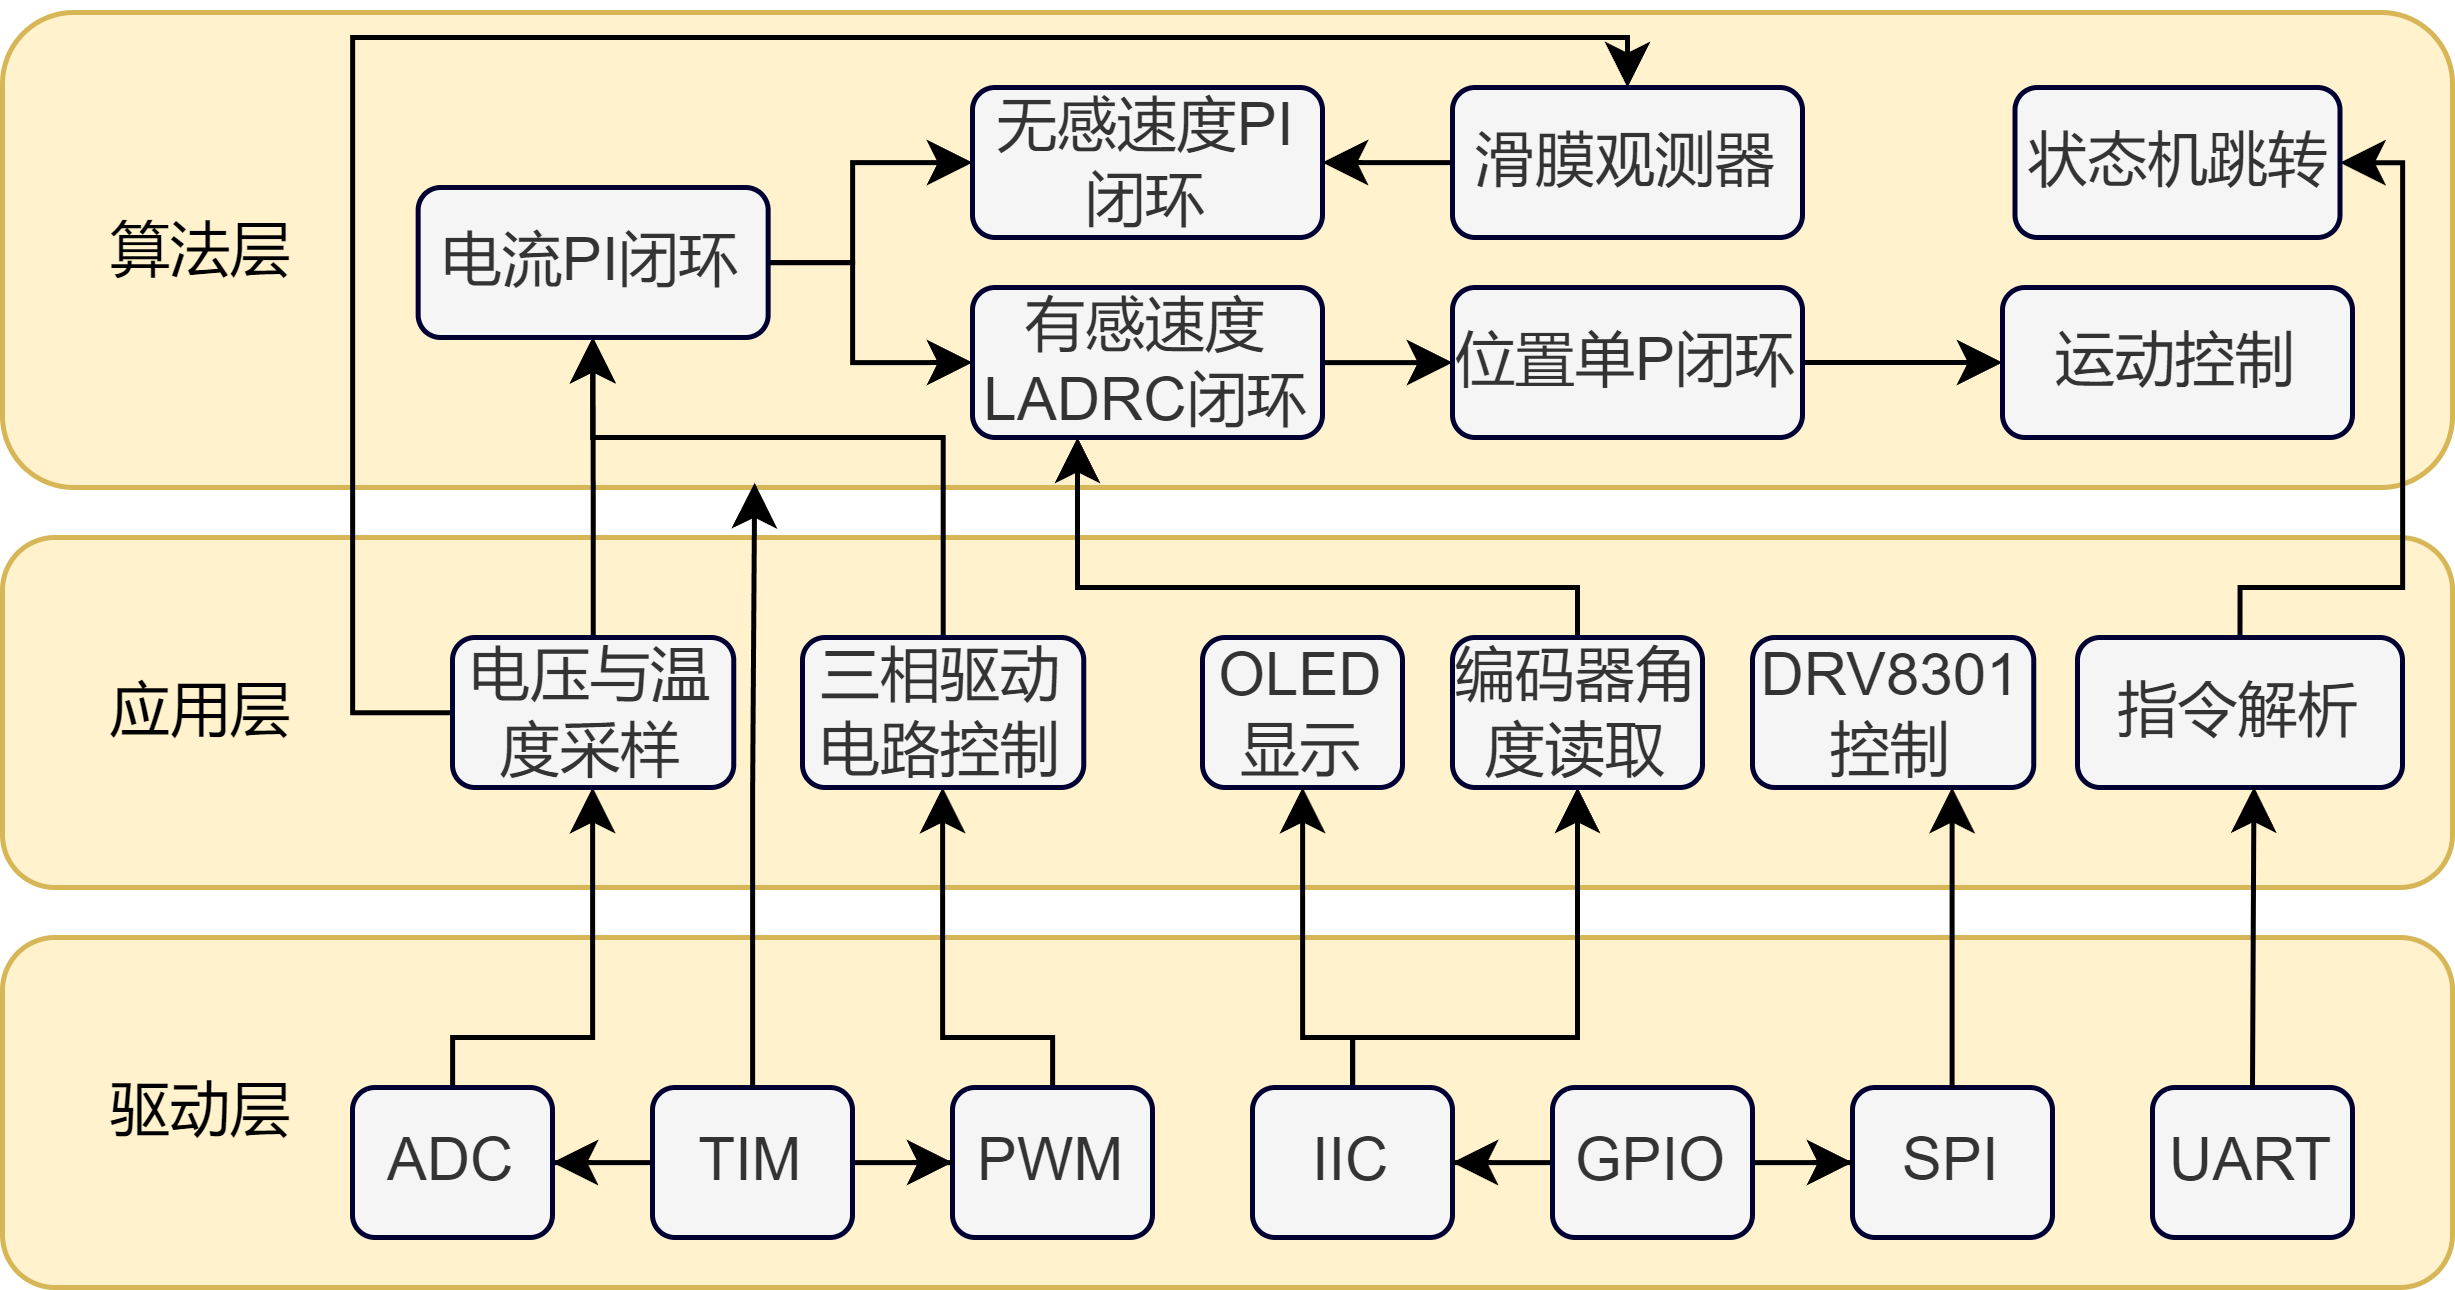
\includegraphics[width=\textwidth]{./picture/软件架构图.drawio.png}
  \caption{软件整体架构图}
  \label{software1}
\end{figure}

定时器中断流程图如图\ref{PRO1}所示,滑膜观测器流程图如图\ref{PRO2}所示。
\begin{figure}[htbp]
  \centering
  \begin{minipage}{0.3\linewidth}
    \centering
    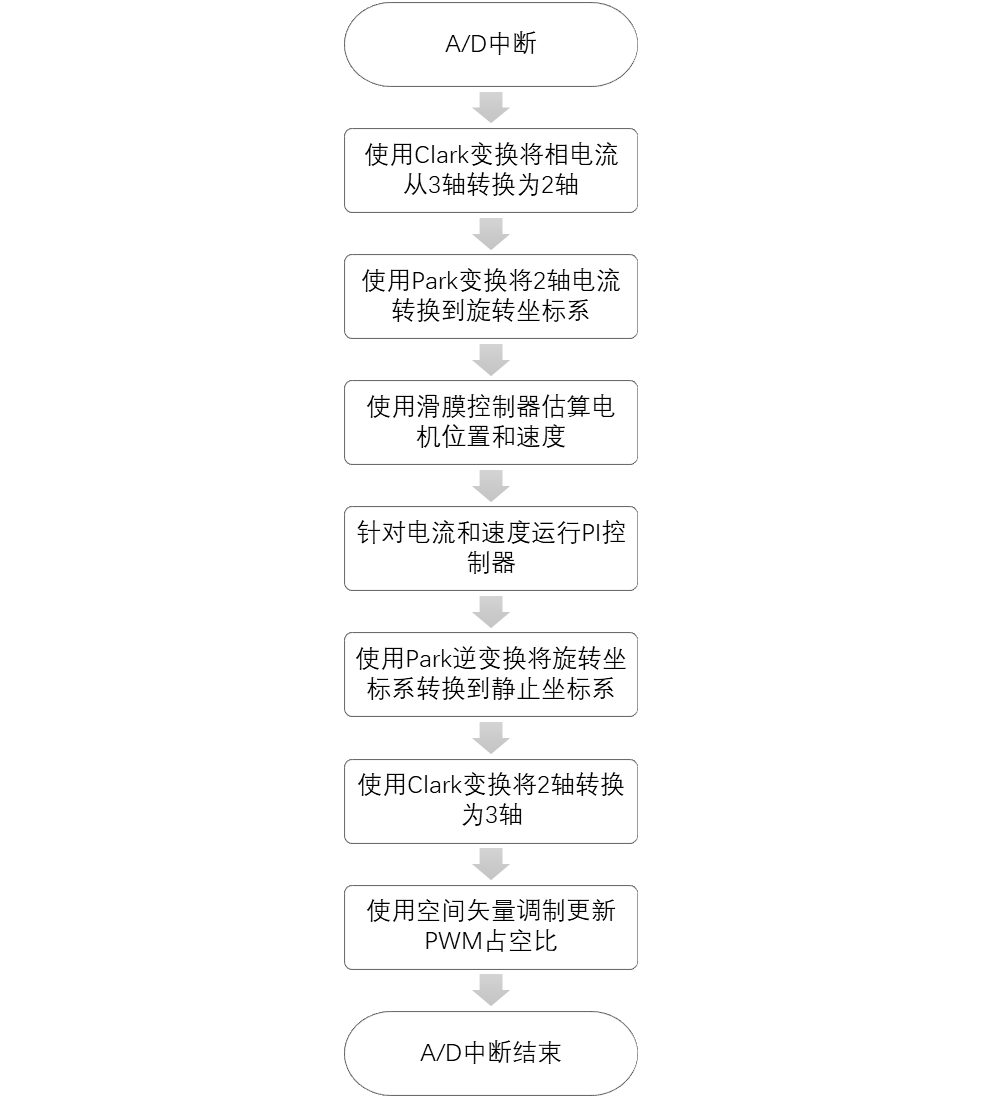
\includegraphics[width=\linewidth]{picture/程序中断流程图.png}
    \caption{程序中断流程图}
    \label{PRO1}%文中引用该图片代号
  \end{minipage}
  \begin{minipage}{0.3\linewidth}
    \centering
    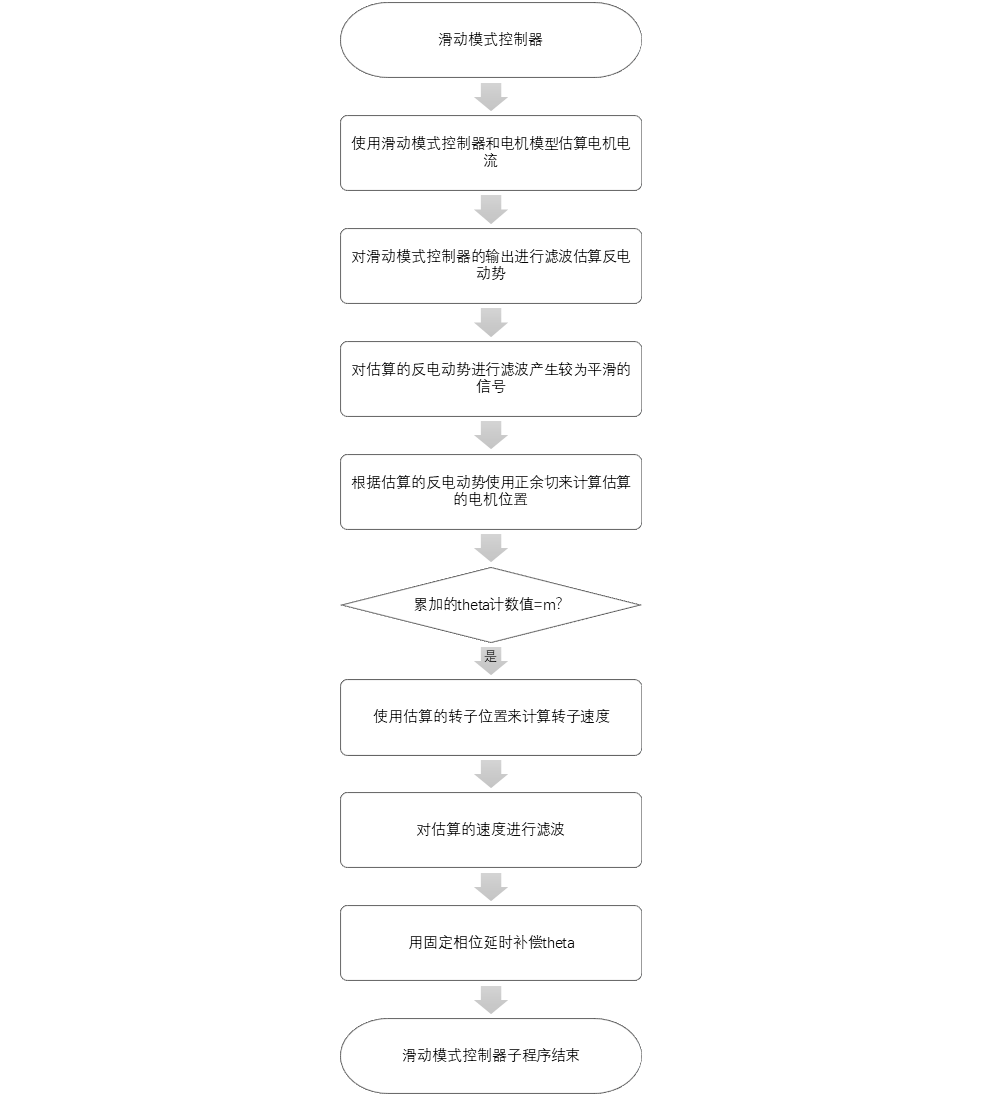
\includegraphics[width=\linewidth]{picture/滑膜观测器流程图.png}
    \caption{滑模观测器流程图}
    \label{PRO2}%文中引用该图片代号
  \end{minipage} 	%\qquad	%让图片换行,
\end{figure}

本章主要讲解软件功能的实现,其中驱动层部分为单片机相关功能开发,不做详细阐述。
算法层中各算法的原理已经在第\ref{原理章}章做了详细阐述,不再赘述。
应用层中,DRV8301和OLED为模块驱动逻辑代码,三相驱动电路控制即包含Clark正逆变换,Park变换和SVPWM输出的解耦控制过程,不做详细阐述。
本章将重点讲解状态机跳转模块,串口指令解析模块,编码器角度读取模块以及其他具有工程参考意义的编码细节。

\subsection{状态机跳转模块}
本项目中,系统有多个模式,由变量MODE进行选择和跳转。
每个模式下有不同阶段的运行状态,由变量STATE进行选择和跳转。
电机驱动的所有运行模式如表\ref{software2}所示:

% \makecell[c]{只把助动词、be动词、情态动词置于主语前;\\ 句首是程度副词}

% \begin{table}[ht]
%     \centering
%     \caption{运行状态说明}
%     \label{software2}
%     \begin{tabular}{cccccc}
%       \toprule
%       & \multicolumn{5}{c}{模式} \\
%       \cmidrule{2-6}
%       & 初始化模式 & 无感速度闭环模式 & 有感速度闭环模式 & 有感位置闭环模式 & 运动控制模式  \\
%       \midrule
%       停止状态 & A & B & C \\
%       运行状态 & I & II& III \\
%       运行完成状态 & I & II& III \\
%       \bottomrule
%       \end{tabular}
% \end{table}

\begin{table*}[!htbp]
  \centering
  \caption{运行状态说明}
  \label{software2}
  \begin{tabularx}{\textwidth}{lXXXXXX}
    \toprule
         & \multicolumn{5}{c}{运行模式}                                                                                      \\
    \cmidrule{2-7}
         & \textbf{初始化模式}           & \textbf{无感速度闭环模式} & \textbf{有感速度闭环模式} & \textbf{有感位置闭环模式} & \textbf{运动控制模式} & 辨识模式 \\
    \midrule
    停止状态 & /                        & 电机停止              & 电机停止              & 电机停止              & 电机停止            & 等待辨识 \\
    运行状态 & /                        & 电机运行              & 电机运行              & 电机运行              & 电机运行            & 正在辨识 \\
    完成状态 & /                        & /                 & /                 & /                 & 到达位置            & 完成辨识 \\
    \bottomrule
  \end{tabularx}%
\end{table*}%

% \subsection{串口指令解析}


\subsection{编码器角度读取模块}
GD32通过SPI读取高精度编码器的原始数据,由于编码器精度较高,且实际过程中会有不可避免的机械抖动,
编码器的原始数据常常会小幅度跳变,为得到稳定的编码器数据,实现精确的控制效果,
本项目在编码器角度读取过程中加入了滑动窗口均值滤波环节。
定义一个大小为n的队列,每次读取出的原始数据插入队列中,在速度环中使用的速度数据为队列中所有值的平均值。


% \subsection{底层电流环}

% \subsection{速度环运行与切换}

% \subsection{位置环}

% \subsection{运动控制环}



\newpage
\section{系统测试与分析}
\subsection{OLED信息显示}
OLED显示信息如图\ref{test1}所示,通过改变代码中的运行状态,可以观测到OLED显示出电机当前的状态。

\begin{figure}[!htbp]
  \centering
  \begin{minipage}{0.29\linewidth}
    \centering
    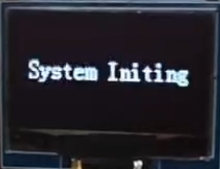
\includegraphics[width=\linewidth]{picture/MODE1.png}
    \caption{系统初始化}
    % \label{chutian1}%文中引用该图片代号
  \end{minipage}
  \begin{minipage}{0.29\linewidth}
    \centering
    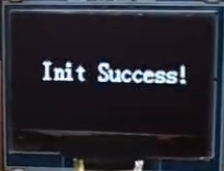
\includegraphics[width=\linewidth]{picture/MODE2.png}
    \caption{初始化成功}
    % \label{chutian2}%文中引用该图片代号
  \end{minipage} 	%\qquad	%让图片换行,
  \begin{minipage}{0.29\linewidth}
    \centering
    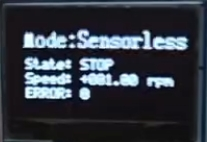
\includegraphics[width=\linewidth]{picture/MODE7.png}
    \caption{无感速度闭环模式}
    \label{chutian3}%文中引用该图片代号
  \end{minipage}
  \begin{minipage}{0.29\linewidth}
    \centering
    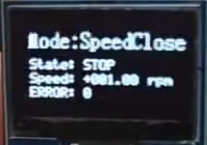
\includegraphics[width=\linewidth]{picture/MODE6.png}
    \caption{有感速度闭环模式}
    \label{test4}%文中引用该图片代号
  \end{minipage}
  \begin{minipage}{0.29\linewidth}
    \centering
    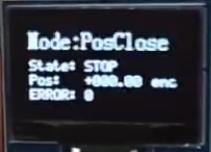
\includegraphics[width=\linewidth]{picture/MODE4.png}
    \caption{位置闭环模式}
    \label{test2}%文中引用该图片代号
  \end{minipage}
  \begin{minipage}{0.29\linewidth}
    \centering
    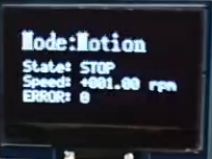
\includegraphics[width=\linewidth]{picture/MODE3.png}
    \caption{运动规划模式}
    \label{test3}%文中引用该图片代号
  \end{minipage}
  \begin{minipage}{0.29\linewidth}
    \centering
    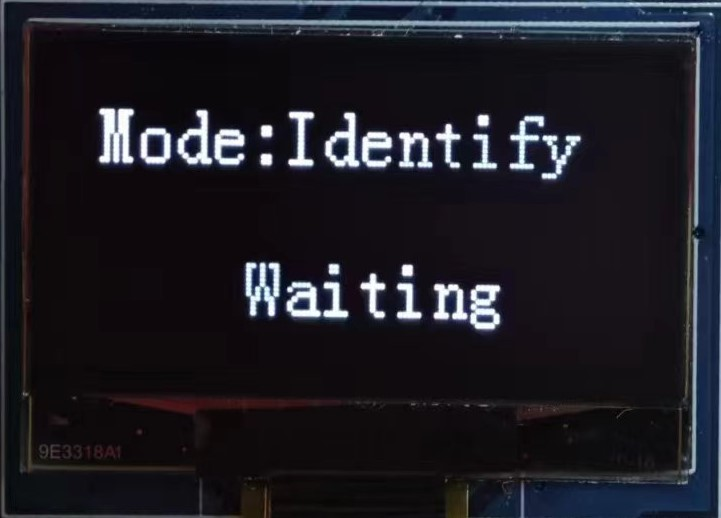
\includegraphics[width=\linewidth]{picture/ID1.jpg}
    \caption{参数辨识模式-等待辨识}
  \end{minipage}
  \begin{minipage}{0.29\linewidth}
    \centering
    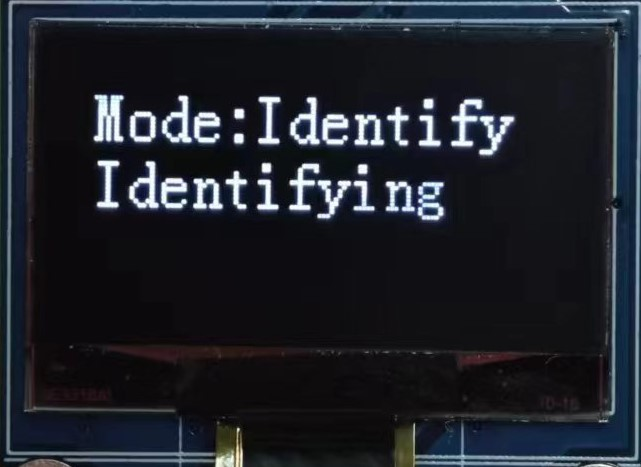
\includegraphics[width=\linewidth]{picture/ID3.jpg}
    \caption{参数辨识模式-正在辨识}
  \end{minipage}
  \begin{minipage}{0.29\linewidth}
    \centering
    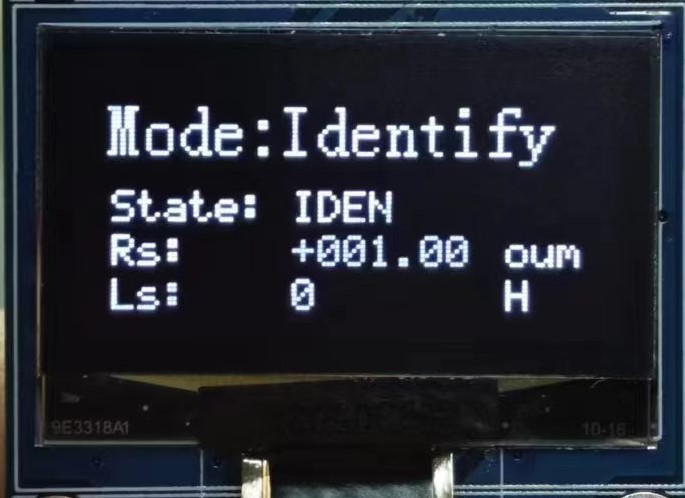
\includegraphics[width=\linewidth]{picture/ID2.jpg}
    \caption{参数辨识模式-辨识完成}
    \label{test6}%文中引用该图片代号
  \end{minipage}
  \caption{OLED信息显示测试}
  \label{test1}
\end{figure}
从图\ref{test3}和图\ref{test2}可以看出,显示屏中,
第一行显示当前的运行模式,第二行显示当前的运行状态。
第三行显示速度,单位为转每分钟,在无感模式下,该值为滑模观测器的估计值,在有感模式下,该值为从编码器解析出的速度值。
在位置闭环模式下,第三行显示位置,其值为编码器的编码值。
第四行会显示错误代码。
在辨识模式下,系统辨识完参数后,会在屏幕中显示电阻大小和电感大小,单位分别为欧姆和亨,如图\ref{test6}所示。

\subsection{参数辨识结果}
辨识出的相电阻是7.11欧,辨识出的线电阻是10.54欧,
对应的相电阻是10.54*2/3=7.02,由此可见辨识结果基本一致。
电阻的辨识过程如图\ref{test100}所示。
\begin{figure}[!htbp]
  \centering
  \begin{minipage}{0.49\linewidth}
    \centering
    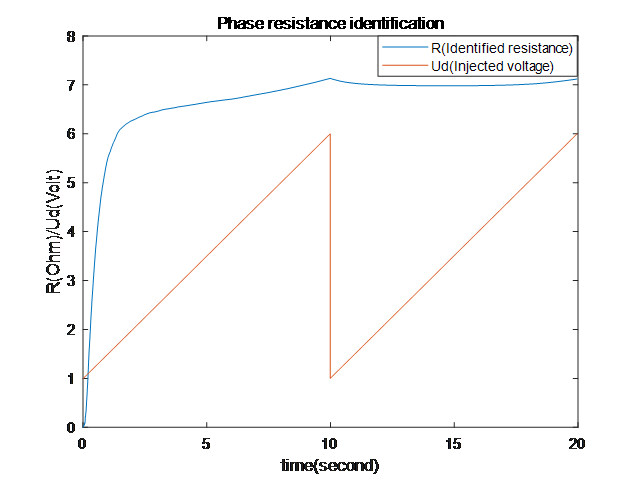
\includegraphics[width=\linewidth]{picture/参数辨识1.png}
    \caption{相电阻辨识过程}
  \end{minipage}
  \begin{minipage}{0.49\linewidth}
    \centering
    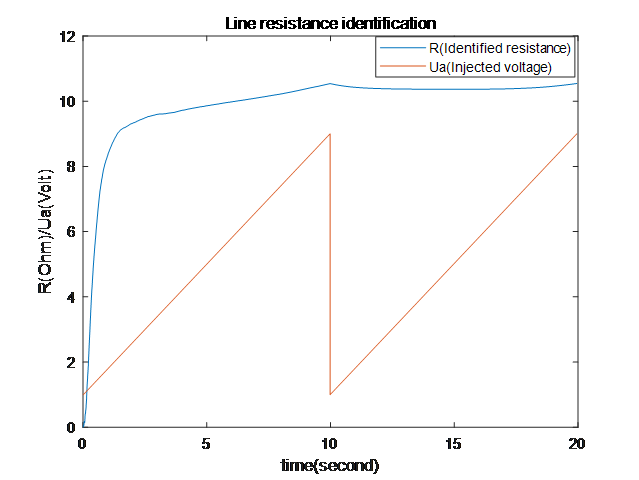
\includegraphics[width=\linewidth]{picture/参数辨识2.png}
    \caption{线电阻辨识过程}
  \end{minipage} 	%\qquad	%让图片换行,
  \caption{电阻辨识过程}
  \label{test100}%文中引用该图片代号
\end{figure}
电感辨识注入2.5k频4.8v方波,
电感的辨识过程如图\ref{test101}所示
\begin{figure}[!htbp]
  \centering
  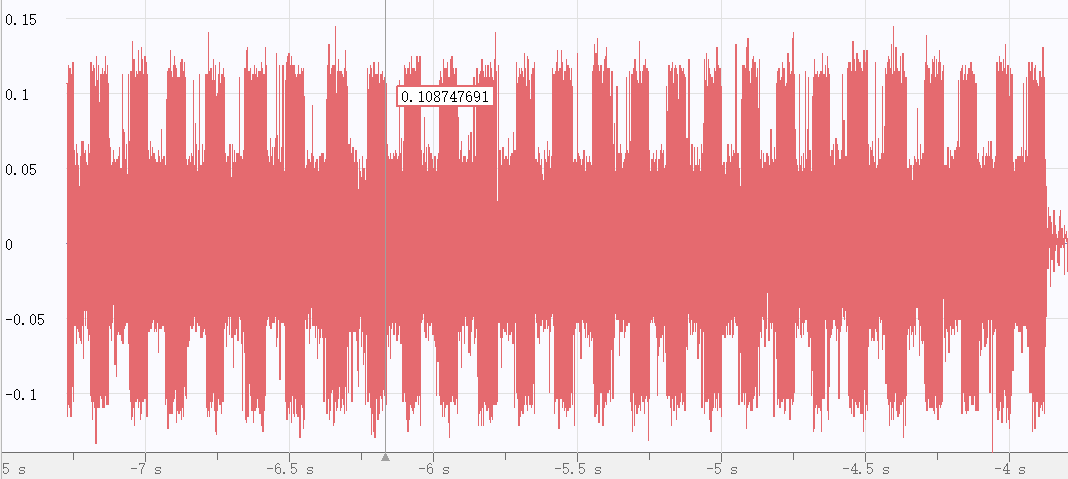
\includegraphics[width=\linewidth]{picture/辨识3.png}
  \caption{电感辨识过程}
  \label{test101}
\end{figure}

\subsection{速度环测试}
在此仅展示无感速度响应曲线,其响应图如图\ref{test102}所示,
图中红线为设定速度,绿线为滑模观测器估计的速度值。
\begin{figure}[!htbp]
  \centering
  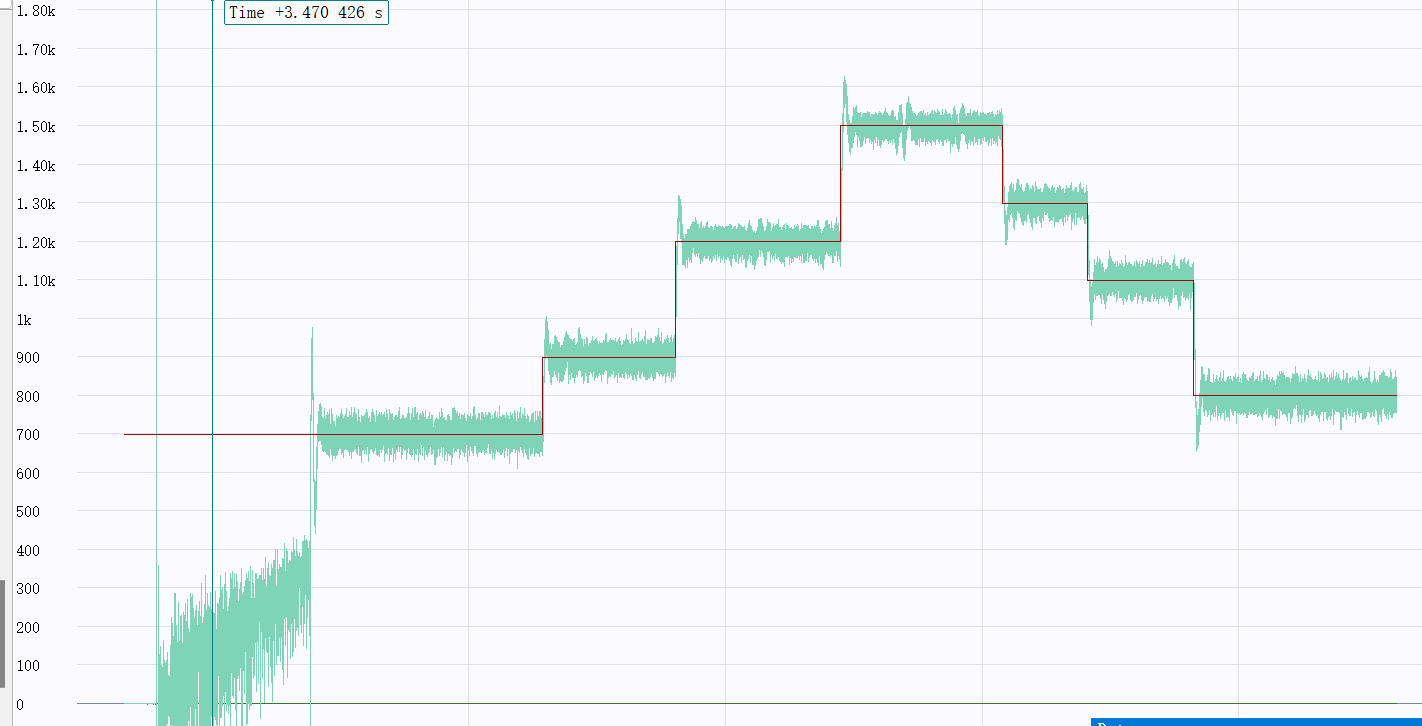
\includegraphics[width=\linewidth]{picture/无感速度波形图.png}
  \caption{无感速度响应图}
  \label{test102}
\end{figure}

% \subsection{电流环测试}
% 电流环响应曲线

% \subsection{速度环测试}
% \subsubsection{无感速度环测试}

% \subsubsection{有感速度环测试}

% \subsection{位置环测试}

% \subsection{运动控制测试}

\clearpage

\newpage
\section{总结}
\subsection{亮点与不足}
本项目融合了有感电机闭环控制和无感电机闭环控制,
且专为机器人关节电机开发了运动控制功能,其制作过程为工业上使用LADRC提供了参考案例。
但不可否认的是,该驱动板还未考虑到更多复杂的工况,
如低速下的转矩脉动,电机末端振动等,这些都是未来的研究方向。

\subsection{未来工作}
硬件电路优化上,半桥刹车电路的电流采样部分,使用了低端接法,但采用了高端电流采样器AD8418。
在实际实验测试过程中,发现刹车电阻的控制并不需要如此高精度的电流采样方案。
因此,后续工作中可以使用单电源供电的同相比例放大器来替换AD8418实现电流采样功能,以此降低驱动器成本。

软件代码开发上,可增加USB通信,CAN通信以满足多样的控制需求\cite{Rohman2021}。
未来将着重开发各类通信协议的ROS接口,以满足各类机器人的电机控制的需求。

特殊工况的优化上,如转矩脉动,在线参数辨识等,希望能借助神经网络\cite{Zhao2022}等技术解决难题。
道阻且长,行则将至,希望这次的比赛是起点而不是终点,希望未来能持续为中国的机器人事业做出贡献。




% % 图表示例
% \newpage
% \section{图表示例}

% 好的,我局的没问题
% 脚注示例
% 正文中引用的例子\footnote{作者, 题目, 出版要素。}。

% % 图示例
% \begin{figure}[ht]
%     \centering
%     \includegraphics[width=0.5\textwidth]{example-image}
%     \caption*{图1-1 示例图题}
%     \label{fig:example}
% \end{figure}

% % 表示例
% \begin{table}[ht]
%     \centering
%     \caption{ 示例表题}
%     \label{tab:example}
%     \begin{tabular}{|c|c|}
%         \hline
%         项目 & 内容 \\
%         \hline
%         示例 & 数据 \\
%         \hline
%     \end{tabular}
% \end{table}

% 参考文献
\newpage
% \begin{thebibliography}{99}
%     \bibitem{ref1} 作者, 题目, 出版要素.
%     \bibitem{ref2} 作者, 题目, 出版要素.
% \end{thebibliography}

\bibliographystyle{unsrt}
% \bibliography{Cogging.bib}\ %IEEEabrv instead of IEEEfull
\bibliography{references.bib}\ %IEEEabrv instead of IEEEfull



\end{document}
